%\documentclass[aps,prl,preprint]{revtex4-1}
\documentclass[aps,prb,showpacs,preprintnumbers,amsmath,amssymb,superscriptaddress,twocolumn]{revtex4}
%\usepackage{amsmath,amsfonts,amssymb}
\usepackage{graphicx}
\usepackage{comment}
%\usepackage{subcaption}
\usepackage{hyperref}
\usepackage{braket}

\newcommand{\midrule}{\hline}
\newcommand{\bottomrule}{\hline\hline}
\newcommand{\bs}{\boldsymbol}
\newcommand{\tr}{\text{tr}}

\usepackage{xcolor}

\newcommand{\up}{\uparrow}
\newcommand{\down}{\downarrow}

\usepackage{esint}
\makeatletter
%% make esint definition in line with amsmath
\@for\next:={int,iint,iiint,iiiint,dotsint,oint,oiint,sqint,sqiint,
  ointctrclockwise,ointclockwise,varointclockwise,varointctrclockwise,
  fint,varoiint,landupint,landdownint}\do{%
    \expandafter\edef\csname\next\endcsname{%
      \noexpand\DOTSI
      \expandafter\noexpand\csname\next op\endcsname
      \noexpand\ilimits@
    }%
  }
\makeatother

% David edits 2018/12/09
%  1. Say what is there, ignore what is not.
%   eg1: ... is the ppc, which is defined as the difference ... -> ... is the difference ...
%   eg2: ... use symmetry in the crystal ... no symmetry in the liquid ... -> ... use symmetry in the crystal ...
%   eg3: 

\begin{document}
\title{Quantum Monte Carlo Compton profiles of solid and liquid lithium}
\author{Yubo Yang}
\affiliation{Department of Physics, University of Illinois, Urbana, Illinois 61801, USA}
\author{Nozomu Hiraoka}
\affiliation{National Synchrotron Radiation Research Center, Hsinchu, 30076, Taiwan}
\author{Kazuhiro Matsuda}
\affiliation{Graduate School of Science, Kyoto University, Kyoto 606-8502, Japan}
\author{Markus Holzmann}
\affiliation{LPTMC, Université Pierre et Marie Curie and CNRS, 75005 Paris, France and LPMMC,
Université Grenoble I and CNRS, 38042 Grenoble, France}
\author{David M. Ceperley}
\affiliation{Department of Physics, University of Illinois, Urbana, Illinois 61801, USA}
\date{\today}
\begin{abstract}
We computed the Compton profile of solid and liquid lithium using quantum Monte Carlo (QMC) and compared with recent experimental measurements obtaining excellent agreement. Importantly, we find it necessary to explicitly include both the valence and the core electrons for quantitative accuracy. To account for disorder effects, we sampled finite-temperature configurations using molecular dynamics (MD), then performed diffusion Monte Carlo (DMC) simulations on each configuration. We used Slater-Jastrow wavefunction and grand-canonical twist-averaged boundary condition. QMC pseudopotential correction was derived from an all-electron DMC simulation of the perfect crystal. Our calculations provide the first all-electron QMC benchmark for the Compton profile of lithium crystal. We also report pseudopotential-corrected QMC Compton profiles under both liquid and solid conditions.
\end{abstract}
\pacs{}
\maketitle

\section{Introduction} \label{sec:intro}

Accessible to both theory and experiment, the Compton profile is a bulk-sensitive probe of the electronic structure of a material. Under the ``impulse approximation''~\cite{Eisenberger1970}, the double differential cross section of inelastic light scattering is directly proportional to the Compton profile, which is the radon transform of the electronic momentum distribution along the scattering vector. The directional Compton profile along z is
\begin{equation}
J(p_z) = \iint dk_x dk_y ~ n(k_x, k_y, k_z=p_z),
\end{equation}
where $n(\bs{k})$ is the electronic momentum distribution.
Since the pioneering work of Eisenberger et. al.~\cite{Eisenberger1970,P.EisenbergerL.LamP.M.Platzman1972}, many Compton scattering experiments have been performed on simple metals such as Li~\cite{Sakurai1995, Schulke1996,Chen1999,Sternemann2001,Tanaka2001}, Be~\cite{Hamalainen1996,Huotari2000}, Na~\cite{Huotari2010} as well as more complicated materials. Accompanying the scattering experiments are numerous theoretical calculations using different electronic structure theories including density functional theory (DFT)~\cite{Sakurai1995,Schulke1996,Tanaka2001,Jarlborg1998,Baruah1999,Bross2005,Makkonen2005,Klevak2016,Sekania2018}, QMC~\cite{Filippi1999,Huotari2010}, and GW~\cite{Yasunori1997,Schulke1999,Eguiluz2000,Olevano2012}.
The Compton profiles in ref.~\cite{Sakurai1995,Schulke1996} were compared to DFT results using the local density approximation (LDA) with Lam-Platzman correlation correction~\cite{Lam1974}.
While the Lam-Platzman correction has been shown to be accurate by QMC~\cite{Filippi1999,Schulke2001,Bross2005}, the theoretical Compton profile is still higher at low momenta and lower at high momenta when compared to experiment. In other words, the predicted Compton profile is typically narrower than experiment.

Both theoretical approximation and experimental procedure may be responsible for a significant fraction of the aforementioned discrepancy. On the experiment side, finite momentum resolution and final-state effects~\cite{Sternemann2000,Soininen2001} both broaden the measured Compton profile. On the theory side, the lack of electronic correlation and the use of pseudopotential both narrow the computed Compton profile. Furthermore, many subtle complications may also be responsible for part of the discrepancy. Examples include: multiple scattering correction, background subtraction, thermal expansion, electron-phonon coupling, and relativistic effects.
%Taking the exact Compton profile as the radon transformation of the exact momentum distribution

In this paper, we present much improved QMC calculations on the solid and the liquid state of lithium. Firstly, we use grand-canonical twist-averaging~\cite{Lin2001} to access the momentum distribution at arbitrary momentum while preserving a sharp Fermi surface. We obtain a momentum resolution of 0.040 a.u., which is higher than the 0.068 a.u. achieved previously~\cite{Filippi1999} (It is straight-forward to increase momentum resolution given more computational resources). Secondly, we perform DMC to improve the trial wavefunction. Thirdly, we use all-electron QMC to explore the pseudopotential bias in the Compton profile. We find that the pseudopotential bias is responsible for the majority of discrepancy between pseudopotential QMC and experimental Compton profiles away from the Fermi surface. Fourth and finally, we apply recently developed finite-size correction~\cite{Holzmann2009,Holzmann2011} to obtain the momentum distribution in the thermodynamic limit. Using this improved procedure, we calculate the disorder-averaged Compton profiles for polycrystal and liquid lithium and obtain excellent agreement with recent high-resolution synchrotron experiment [K. Matsuda and N. Hiraoka].

In section \ref{sec:method}, we describe the simulation methods used to obtain the QMC momentum distributions. In section \ref{sec:results}, we show the QMC momentum distributions and the resulting Compton profiles in comparison with experiment. In section \ref{sec:discussion}, we discuss the influence of various physical effects on the momentum distribution in an attempt to explain the remaining discrepancy between QMC and experiment.

\section{Method} \label{sec:method}

Full-core and pseudopotential QMC calculations have been performed on the perfect crystal and disordered configurations. All QMC calculations use the Slater-Jastrow trial wavefunction eq.~(\ref{eq:sj}) with grand-canonical twist-averaged boundary condition.
\begin{align}
\Psi_T = D^{\up} D^{\down} \exp\left[ -\sum\limits_{i<j}^{N} u(\bs{r}_i-\bs{r}_j) - \sum\limits_{i=1}^N \chi(\bs{r}_i) \right],\label{eq:sj}
\end{align}
where $u(\bs{r})$ is the electron-electron Jastrow pair potential and $\chi(\bs{r})$ is the electron-ion Jastrow pair potential, $\bs{r}_i$ being the real-space coordinates of the i$^{th}$ electron. The Slater determinant $D^{\up/\down}$ is composed of single-particle orbitals obtained using Kohn-Sham (KS) DFT with the LDA functional. In the full-core calculation, we remove the approximate electron-ion cusp from the orbitals and re-introduce the exact cusp condition in the Jastrow potential. In the pseudopotential calculation, we treat the lithium atoms as pseudo ions of charge +1. The 1s core electrons are replaced by the BFD pseudopotential~\cite{Burkatzki2007}.  The electron-electron pair potential is expressed as a sum of real-space and reciprocal space parts to accurately describe long-range plasmon fluctuations.

In variational Monte Carlo (VMC), we sample $\vert \psi_T \vert^2$ using Metropolis Monte Carlo and directly calculate properties from the many-body wavefunction. The momentum distribution is calculated using the direct estimator in reciprocal space, first used by McMillan~\cite{W.L.McMillan1965}. In DMC, an ensemble of electron configurations evolve according to the Green's function of the non-relativistic Schr\"odinger equation in imaginary time. Using the trial wavefunction $\psi_T$ as guiding function and nodal reference, the long-time solution samples the mixed distribution $\psi_T\psi_{FN}$, in the limit of infinitesimal time step. $\psi_{FN}$ is the so-called fixed-node ground-state wavefunction. If the node of $\psi_T$ is exact, then $\psi_{FN}$ is the exact ground-state wavefunction.~\cite{Foulkes2001}
%Detailed balance is enforces using Metropolis rejection and time-step error is controlled. Estimators converge to their expectations in the mixed distribution.
The difference between the expectation value of an observable in the fixed-node and the mixed distributions is the mix-estimator bias. %There is no mixed-estimator bias for estimators that commute with the Hamiltonian. The quality of the trial wavefunction can be quantified by the Monte Carlo mean and variance of the total energy in VMC. Further, the change of observables from VMC to DMC can be related to the overlap between the trial and the true ground-state wavefunctions [IE].
We gauge simulation quality by monitoring kinetic, potential, and total energies as well as pair correlation functions, and the momentum distribution. The DMC momentum distribution is linearly extrapolated to remove the mixed-estimator bias. For more details on the computational methods and data processing, see supplementary material.

We use the grand-canonical twist average technique to improve the momentum distribution. A previous QMC calculation~\cite{Filippi1999} used anti-periodic and periodic boundary conditions, with the same number of electrons at each boundary condition (twist). This restricted the accessible momenta to those commensurate with the simulation cell. Further, by keeping the number of electrons constant at all twists, some states outside of the Fermi surface will be occupied at certain twists. In contrast, the grand-canonical twist average technique enforces constant chemical potential at all twists. We adjust the number of electrons at each twist such that no state outside the Fermi surface is occupied. This allows us to sample the momentum distribution at arbitrary momenta while maintaining a sharp Fermi surface. In the perfect crystal, the full-core simulation contains 54 lithium atoms, while the pseudopotential simulations contain 54 or 432 atoms.
%We set the chemical potential to the LDA Fermi energy to reproduce the KS-LDA Fermi surface.
%In both the 54-atom and the 432-atom simulations, we use a dense twist-average grid to set momentum-space resolution to 0.040 a.u., which is higher than the 0.068 a.u. achieved previously with a 686-atom cell~\cite{Filippi1999}. It is straightforward to increase the resolution even further. In the perfect crystal, we use twists in the irreducible wedge of the cubic cell. We also assume time-reversal symmetry to roughly halve the number of necessary calculations. %In disordered configurations, we use half of all twists due to time reversal, but a lack of crystal symmetry.

We use MD with the modified embedded-atom potential (MEAM)~\cite{Baskes1992} to generate the disordered configurations. We sample the canonical distribution with 432 lithium atoms at 330K and 500K for experiments at 298K and 493K, respectively. We elevate the classical MD temperatures to roughly account for quantum fluctuations of the nuclei ~\cite{Filippi1998}.

All calculations have been performed at the same density $r_s=3.25$, consistent with the previous QMC study~\cite{Filippi1999}.
We use LAMMPS~\cite{Plimpton1993} for the MD simulations, QE~\cite{Giannozzi2009,Enkovaara2017} for the DFT calculations, and QMCPACK~\cite{Kim2018} for the QMC calculations. The disordered calculations have been automated using the nexus suite of tools~\cite{Krogel2016}.

\section{Results} \label{sec:results}

In Fig.~\ref{fig:nk}, 1D slices of the QMC valence momentum distributions are shown. The momentum distribution is free-electron-like along the [100] and [111] directions. Along the [110] direction, however, there is a pronounced secondary Fermi surface, which is centered around the Bragg peak of the BCC crystal. The valence profile calculated from the full-core calculation is flatter inside the Fermi surface and has enhanced secondary features when compared to the pseudopotential calculation. To obtain the valence momentum distribution from the full-core QMC calculation (red lines), we remove the momentum distribution of the 1s core electrons. The 1s orbital of the neutral lithium atom is calculated using Hatree-Fock (HF). The most pronounced effect of the pseudopotential is to increase the electronic momentum density inside the Fermi surface, raising $n(0)$ by more than 5\%. In contrast, the effect of increasing system size peaks at the Fermi momentum. The main effect of finite system size is to increase the magnitude of the discontinuity at the Fermi momentum. The effects of pseudopotential and finite system size can be better shown in the momentum distribution differences.

\begin{figure}
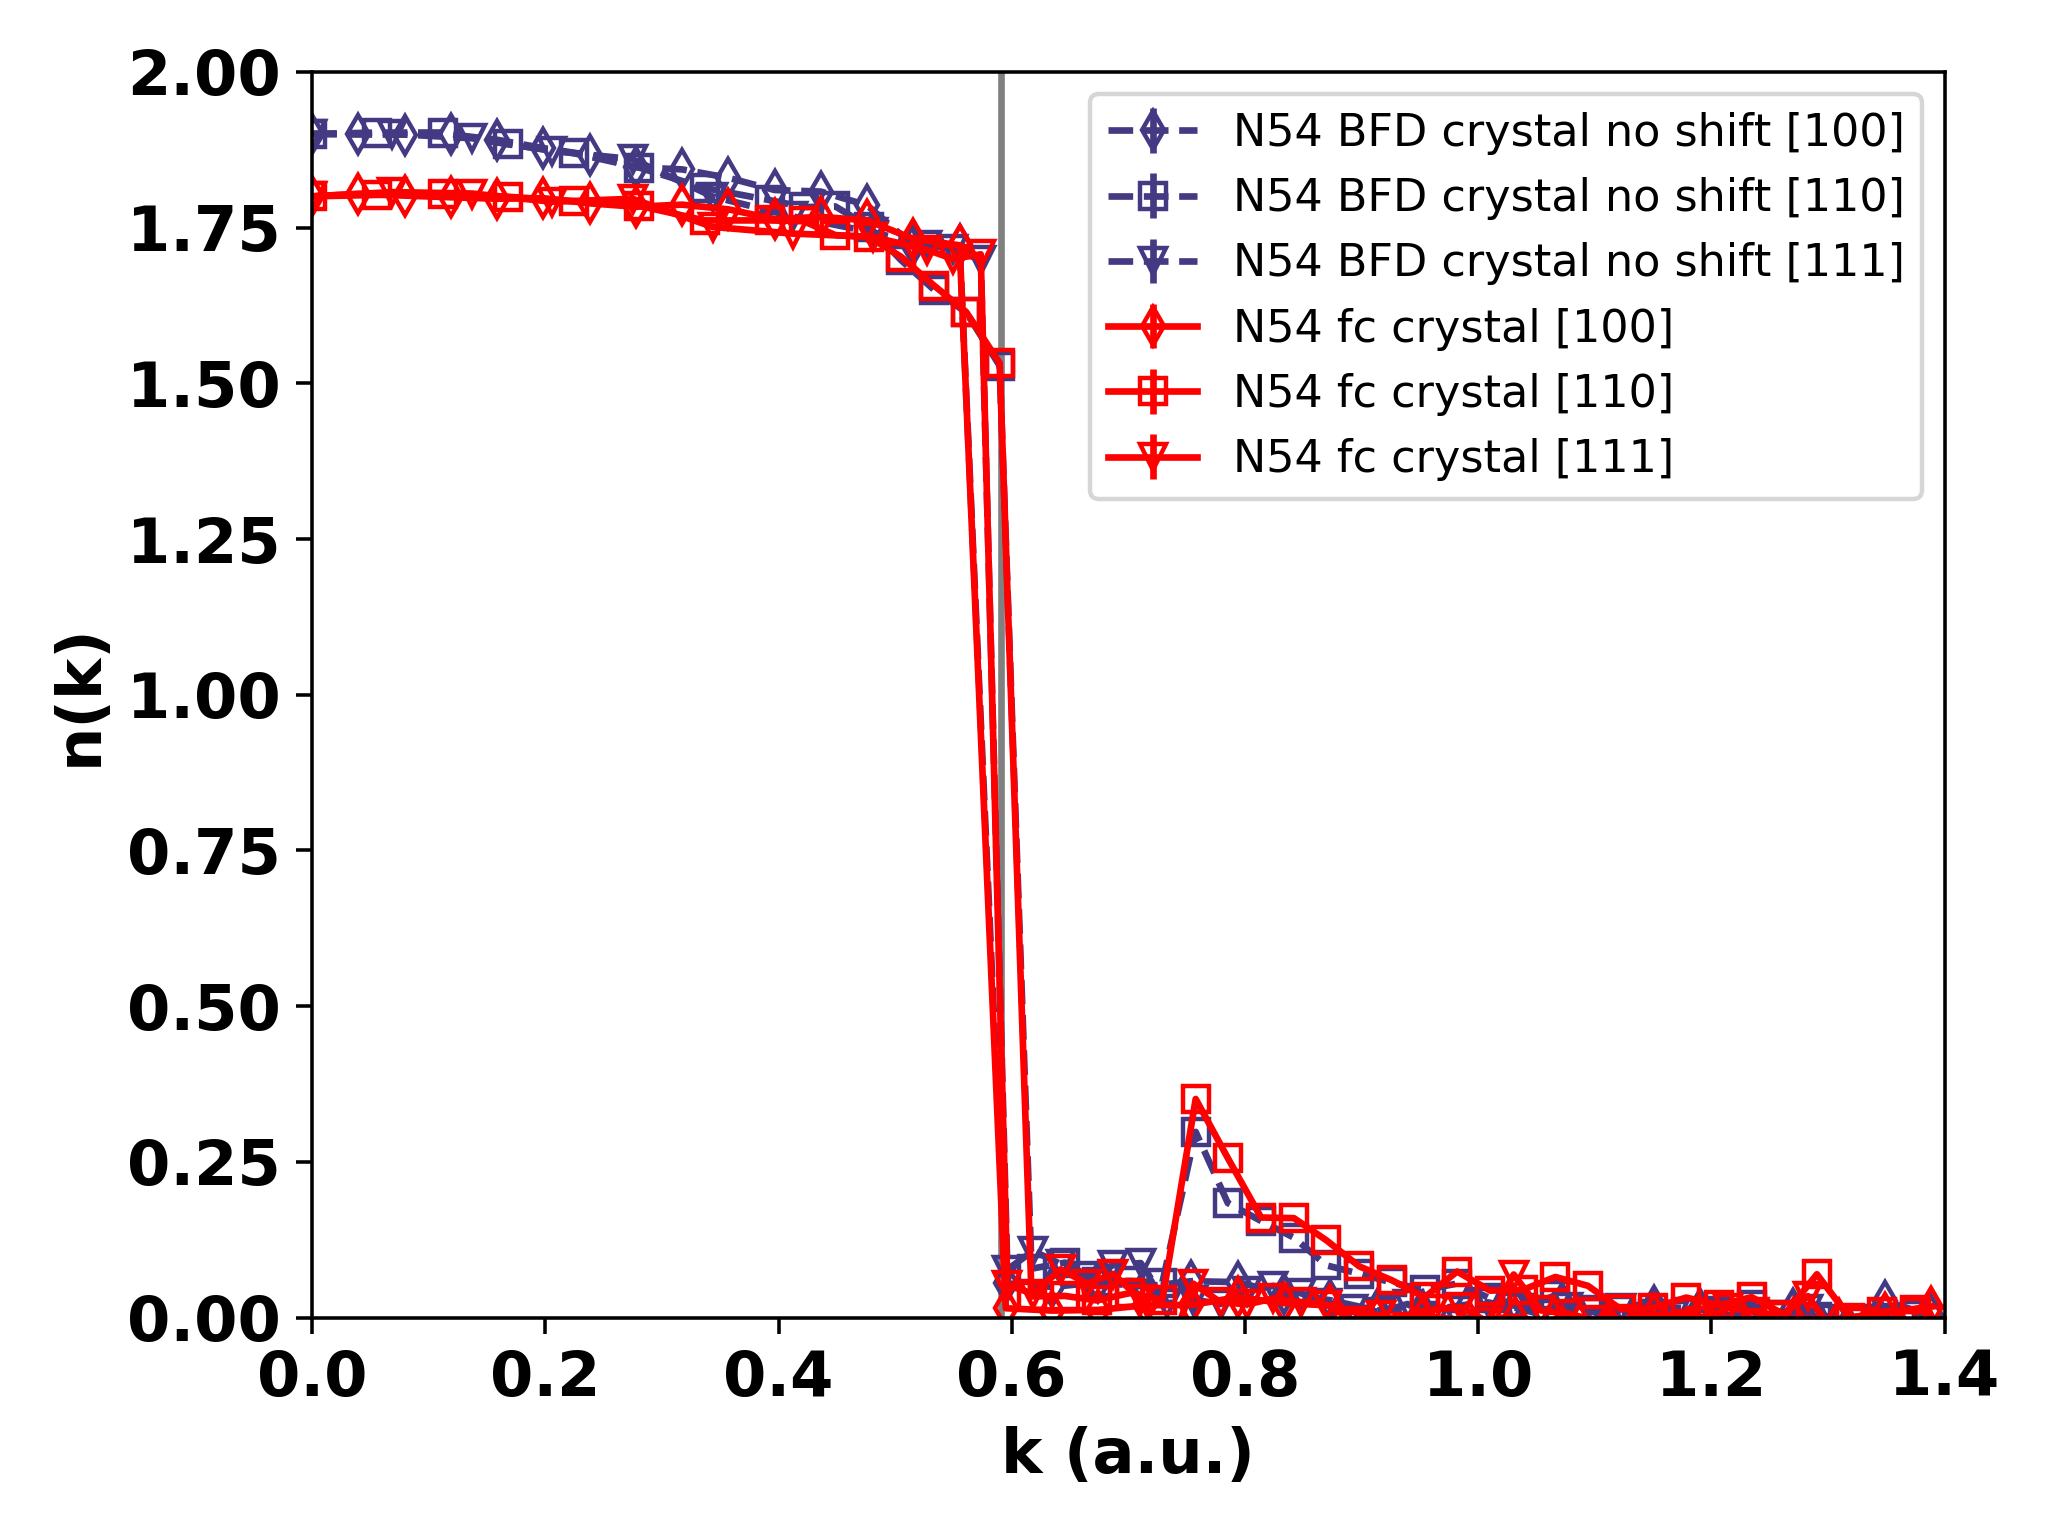
\includegraphics[scale=0.45]{figures/li40_bfd3-n54-nk-ppc}
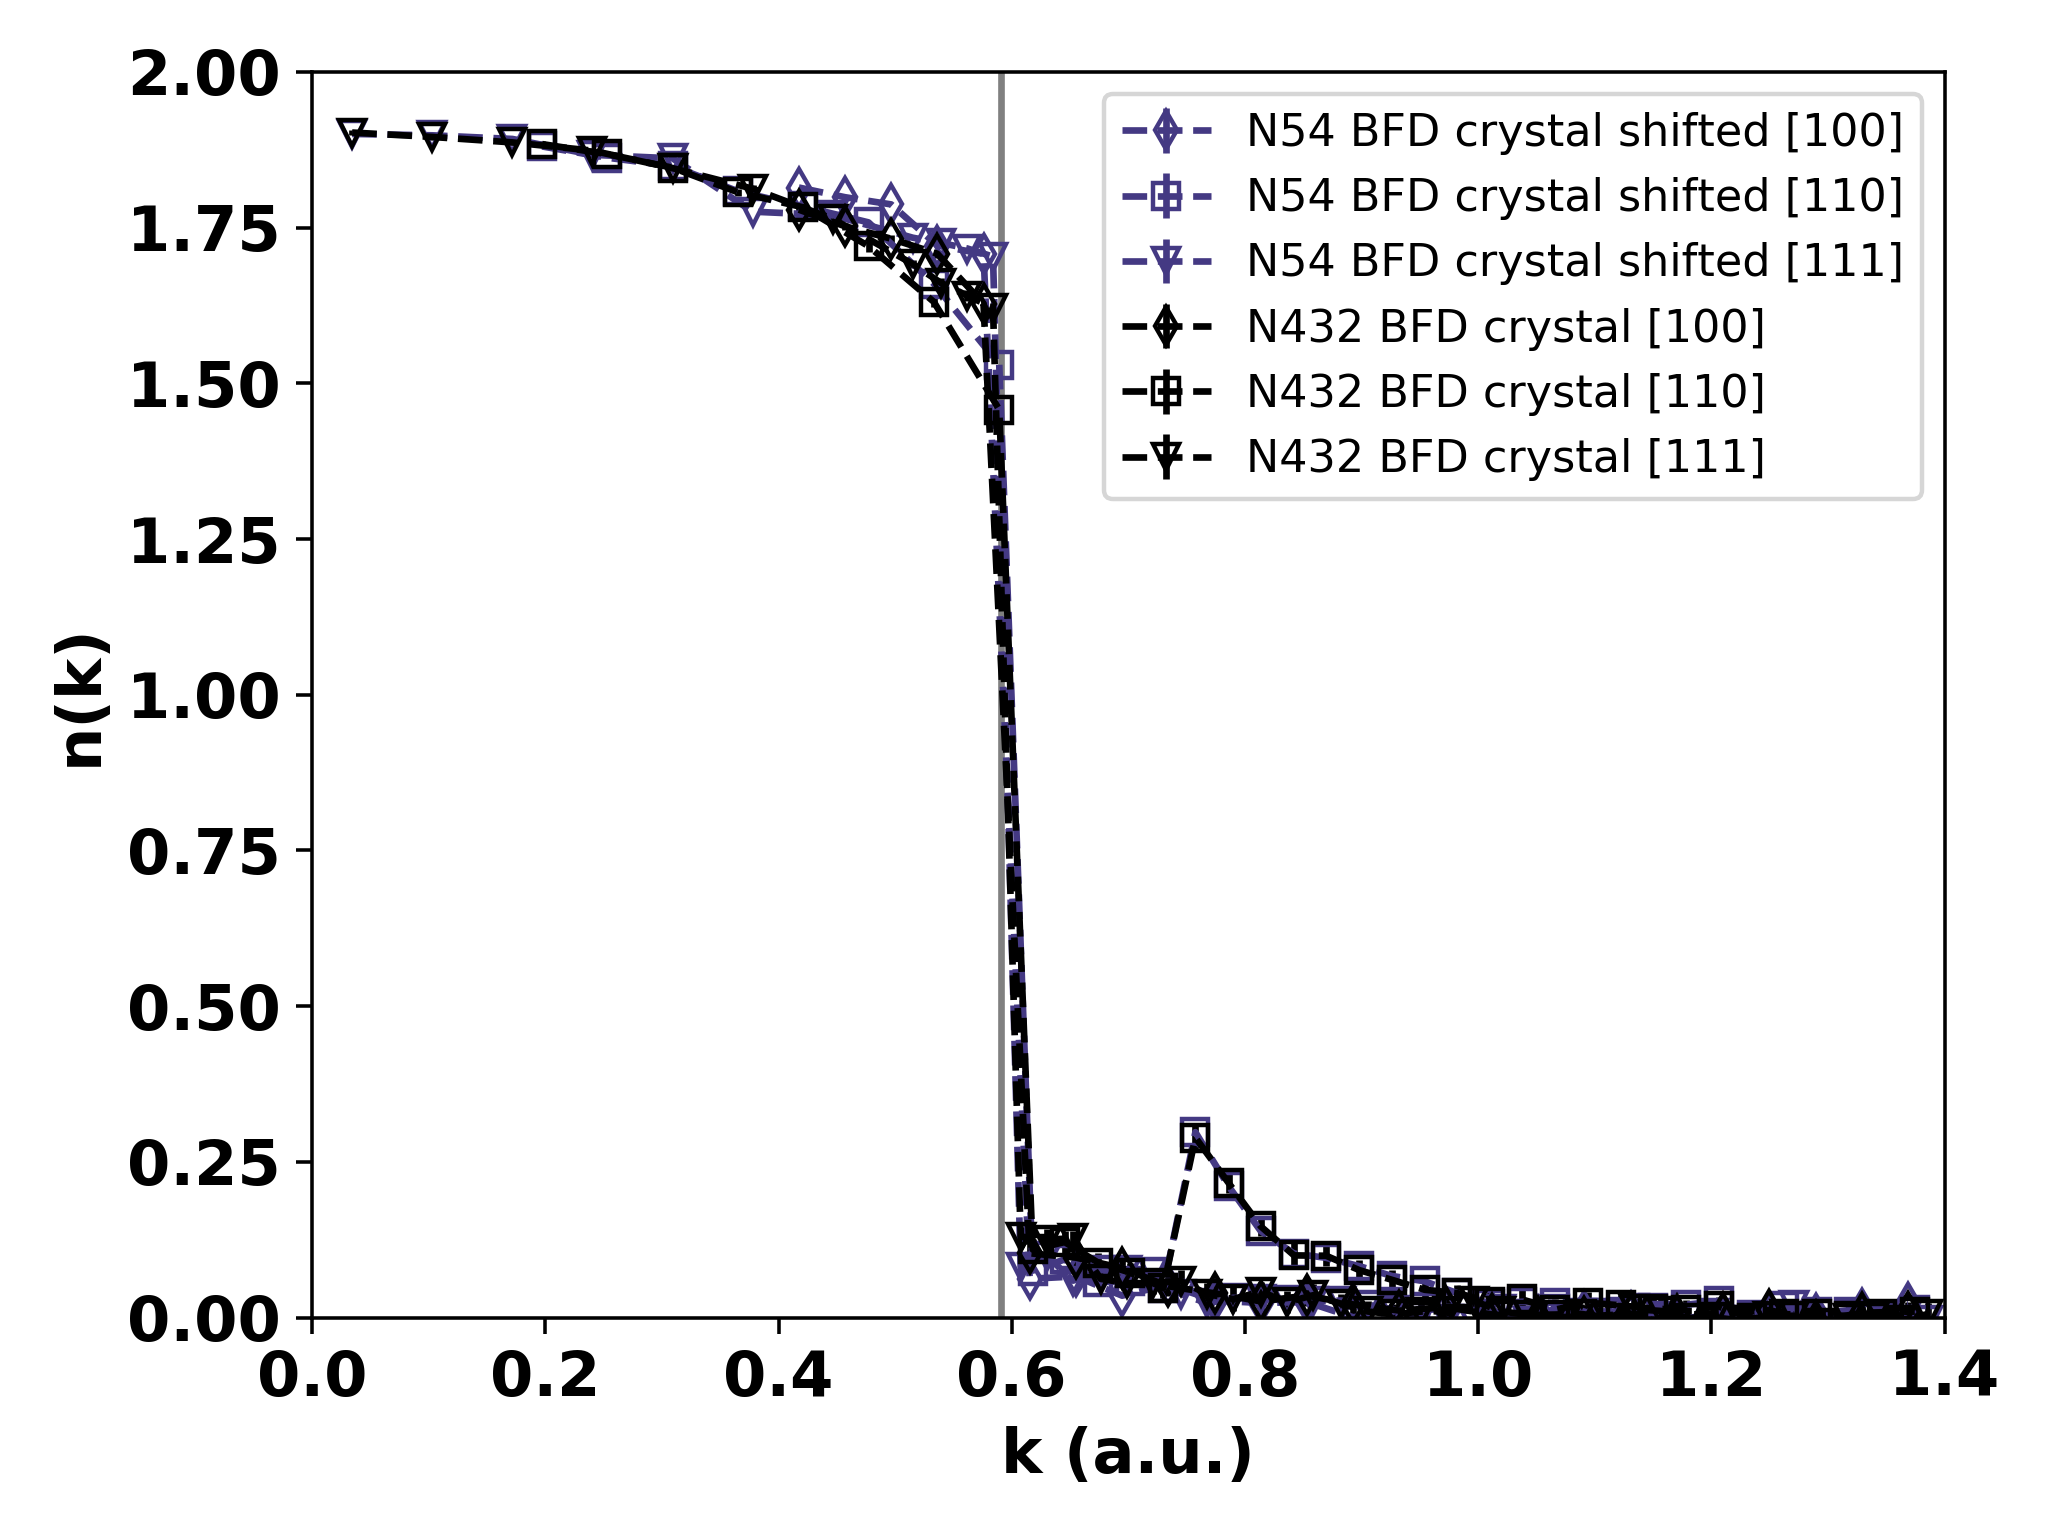
\includegraphics[scale=0.45]{figures/li40_bfd3-nk-fsc}
\caption{Momentum distribution of valence electrons in lithium BCC crystal. The top panel compares pseudopotential (purple) to full-core (red) result.
%The core contribution to the momentum distribution is calculated from HF 1s orbital for the neutral lithium atom.
The bottom panel compares 54-atom (purple) to 432-atom (black) pseudopotential results. The vertical gray line marks the Fermi momentum of the homogeneous electron gas at the same density.\label{fig:nk}}
\end{figure}

In Fig.~\ref{fig:dnk}, we show two sets of momentum distribution differences in direct correspondence with Fig.~\ref{fig:nk}. The first is the difference between full-core and pseudopotential momentum distributions. This difference can be considered a pseudopotential correction (PPC). The PPC is largest inside the Fermi surface. It has a parabolic shape and a discontinuity at the Fermi momentum. The PPC is mostly negative along the [100] and [111] directions. However, it shows positive peaks near the secondary Fermi surface along the [110] direction. The second set of differences are taken between the 432-atom and 54-atom pseudopotential calculations. This difference can be considered a finite-size correction (FSC). The FSC peaks at the Fermi surface and is essentially zero at high momenta. The momentum distribution differences are spherically-averaged and integrated to obtain PPC and FSC for the spherically-averaged Compton profile.

\begin{figure}
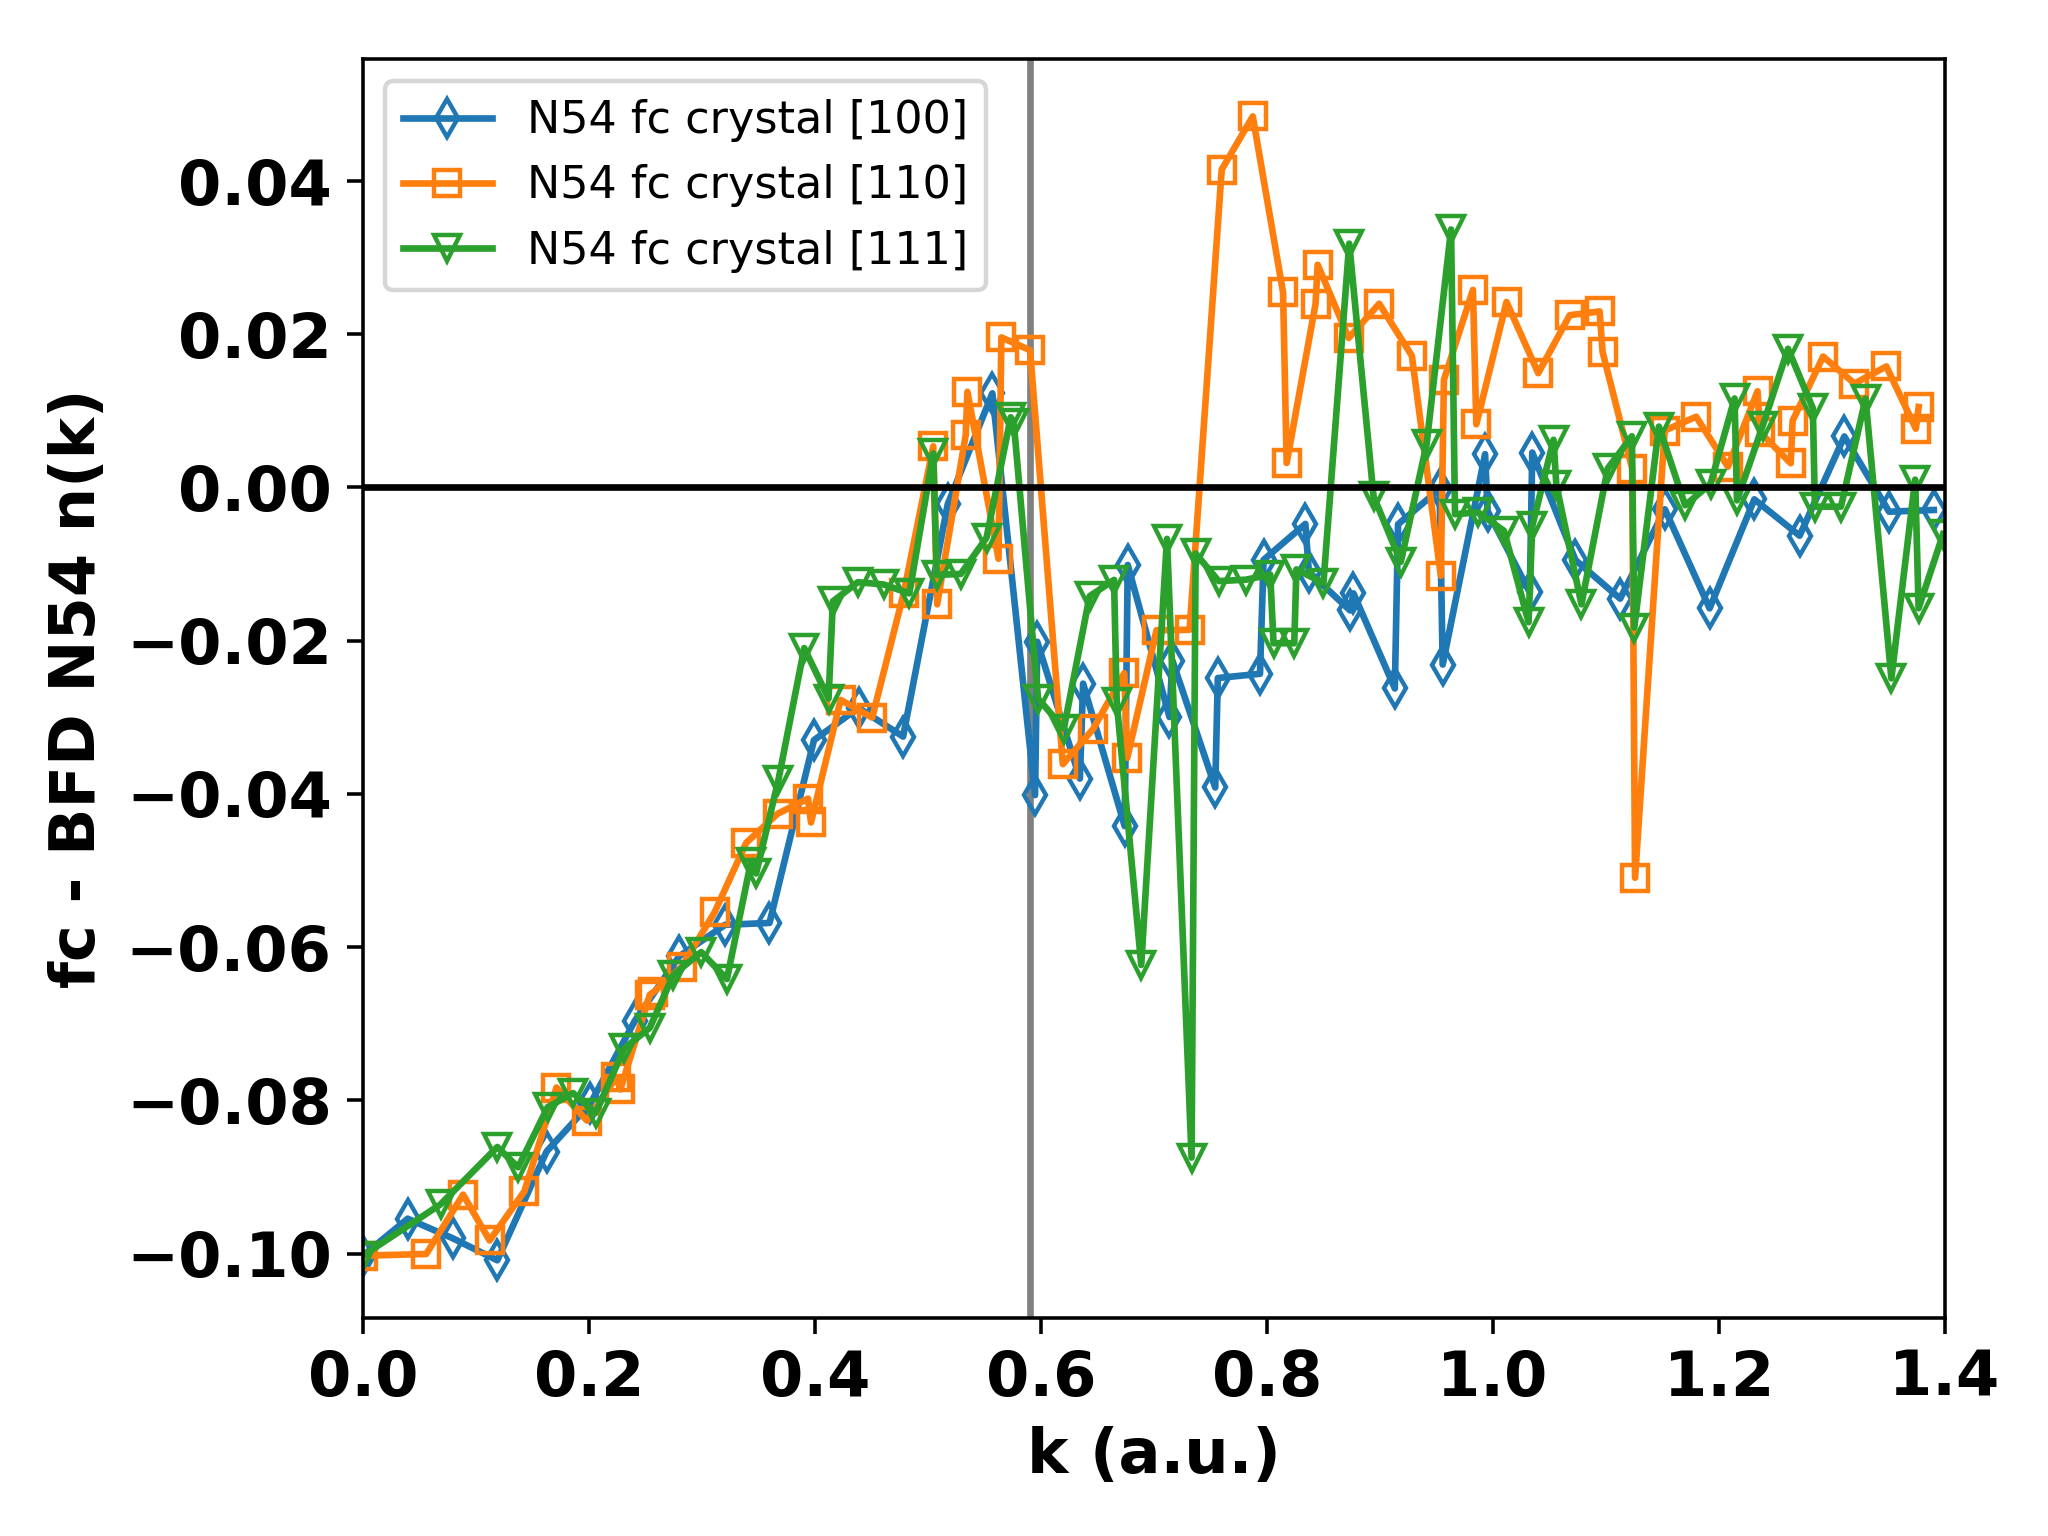
\includegraphics[scale=0.45]{figures/li40_bfd3-dnk-ppc}
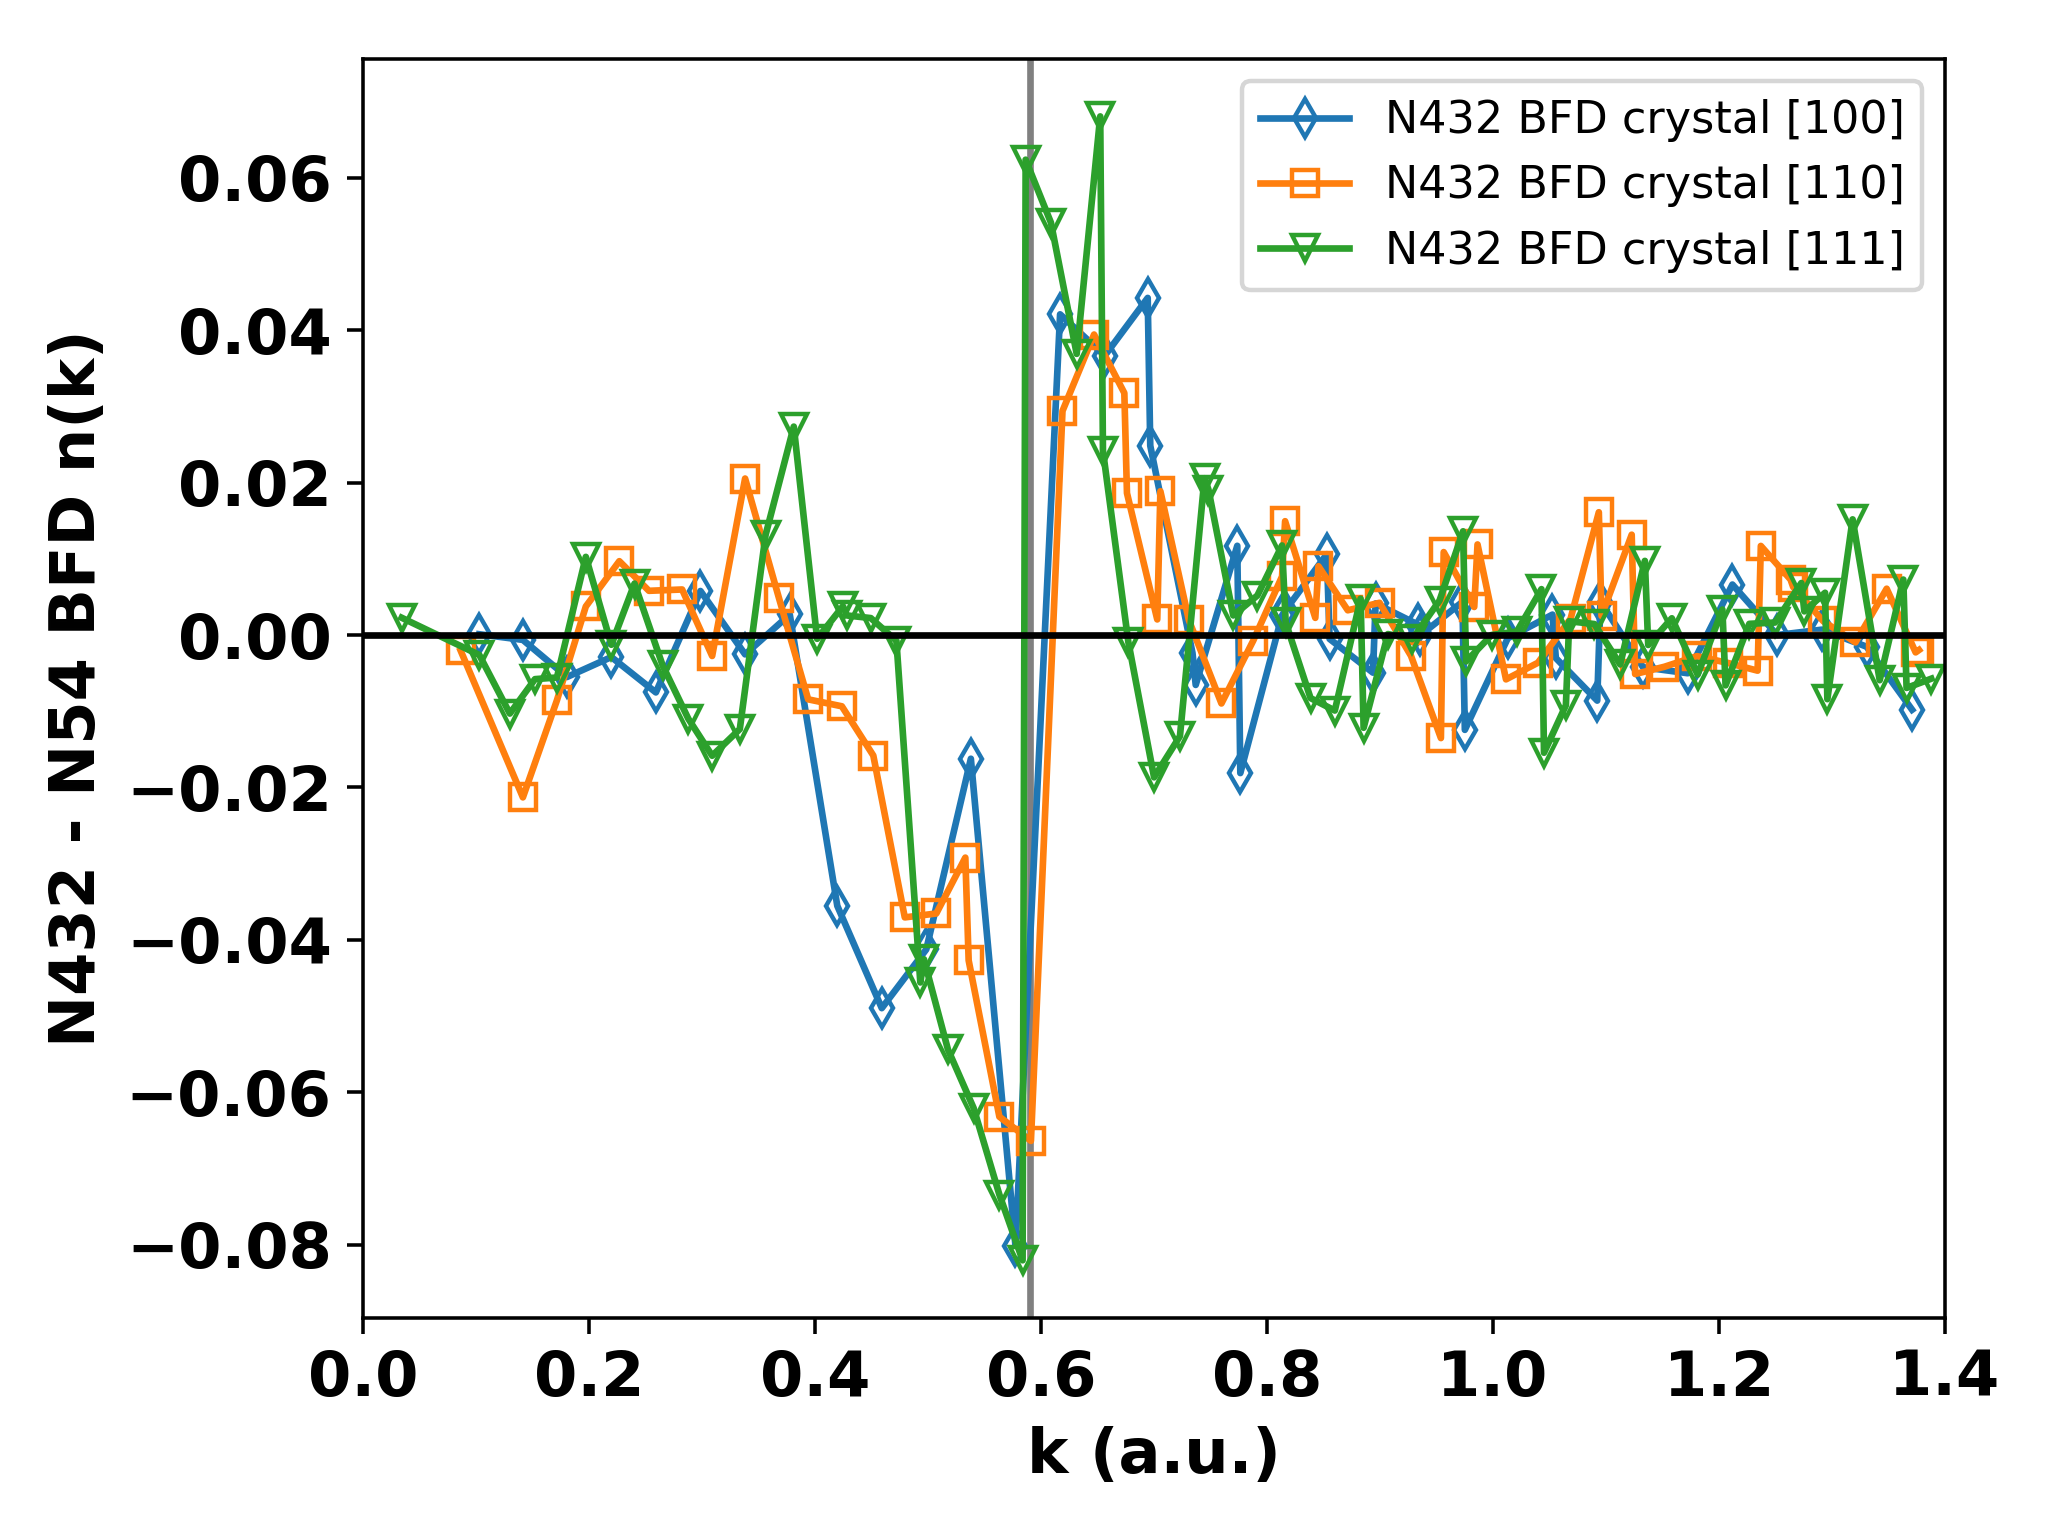
\includegraphics[scale=0.45]{figures/li40_bfd3-dnk-fsc}
\caption{Pseudopotential and finite-size corrections of the momentum distribution of valence electrons in lithium BCC crystal. The top panel is the difference between full-core and pseudopotential results. The bottom panel is the difference between the 432-atom and 54-atom pseudopotential results. The vertical gray line marks the Fermi momentum of the homogeneous electron gas at the same density.\label{fig:dnk}}
\end{figure}

%We derive a finite-size correction for the Compton profile from the difference between the 54-atom and 432-atom pseudopotential momentum distributions. The difference is spherically averaged, then integrated to obtain a correction for the isotropic Compton profile. This correction is added to the spherically-averaged full-core Compton profile, which is then smeared using convolution to approximately account for the effects of finite experimental resolution and interaction in the final state. Finally, we subtract the same core signal as the experiment (Hatree-Fock 1s) to produce the final valence Compton profile in Fig.~\ref{fig:crystal-vcp}.

In Fig.~\ref{fig:crystal-vcp}, we show our best QMC Compton profile in the crystal as the red line. It is the spherically-averaged Compton profile from the full-core calculation with FSC applied. Further, we convolved the QMC Compton profile with a model function (see discussion) to approximately account for experimental resolution and final state effects. The full-core QMC profiles agrees very well with the most recent experiment away from the Fermi surface.
Notice that the Compton profile reported by Filippi and Ceperley \cite{Filippi1999} is closer to our full-core than to our pseudopotential result. This is because they accounted for proper core-valence orthogonalization using full-core LDA. Pseudopotential QMC was used to estimate the correlation correction, rather than directly provide the Compton profile.
%their reported QMC Compton profile effectively includes an LDA pseudopotential correction. Specifically, full-core LDA + QMC correlation correction = pseudopotential QMC + LDA pseudopotential correction.

\begin{figure}
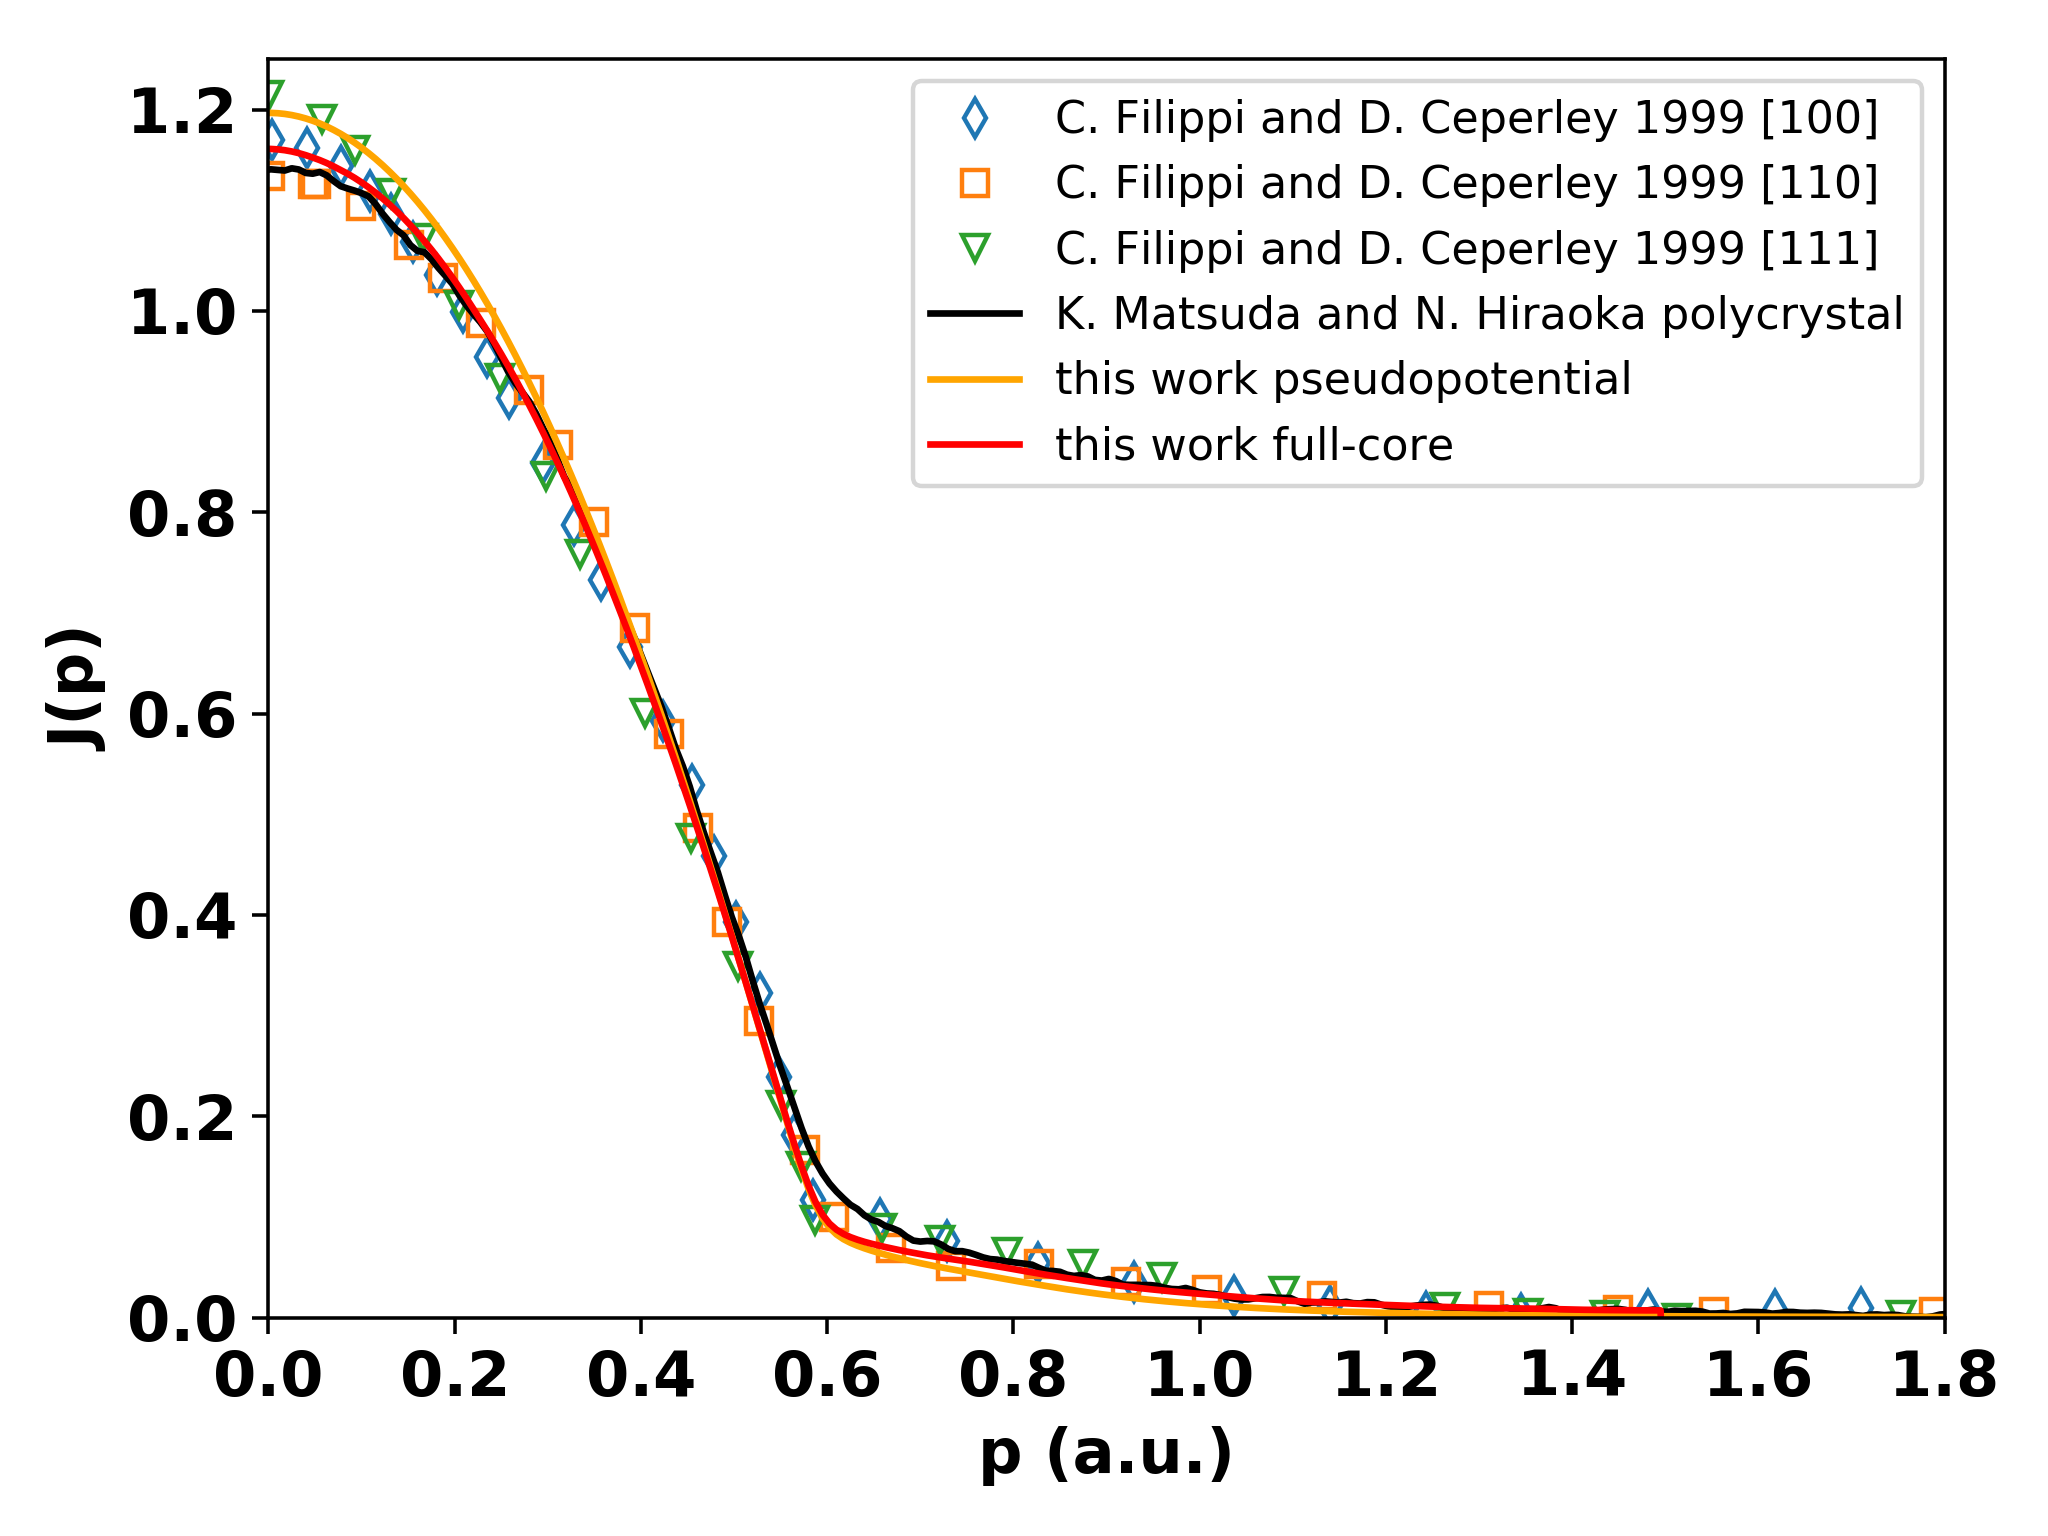
\includegraphics[scale=0.48]{figures/li40_fc7-vcp}
\caption{Valence Compton profile of lithium BCC crystal at $r_s=3.25$. The red solid line is our best result derived from the spherically-averaged momentum distribution of the full-core QMC calculation. The orange curve is our best pseudopotential QMC calculation. The black curve is the most recent experiment on polycrystal lithium. The symbols are QMC Compton profiles from Filippi and Ceperley~\cite{Filippi1999}. The [100], [110], and [111] directions correspond to diamond, squares, and triangles, respectively.\label{fig:crystal-vcp}}
%The raw 3D $n(\bs{k})$ from the 54-atom all-electron DMC was processed in 3 steps A finite-size correction was added from N432 - N54 pseudopotential QMC \textcolor{red}{Compton profiles}. 
\end{figure}

Taking our best QMC Compton profile (red line in Fig.~\ref{fig:crystal-vcp}) as reference, we show the remaining difference between the QMC and the experiment Compton profiles as the black curve in Fig.~\ref{fig:crystal-ppc}. We also show the effect of using various approximations in the calculation of $J(p)$. As shown in Fig.~\ref{fig:crystal-ppc}, three corrections are considered: pseudopotential, finite-size, and convolution. All three lower the value of $J(0)$, bringing it closer to experiment. The pseudopotential correction is dominant over the convolution and finite-size corrections. Further, the pseudopotential correction is the only one that contributes at momenta far above the Fermi momentum ($p>0.75$ a.u.).

\begin{figure}
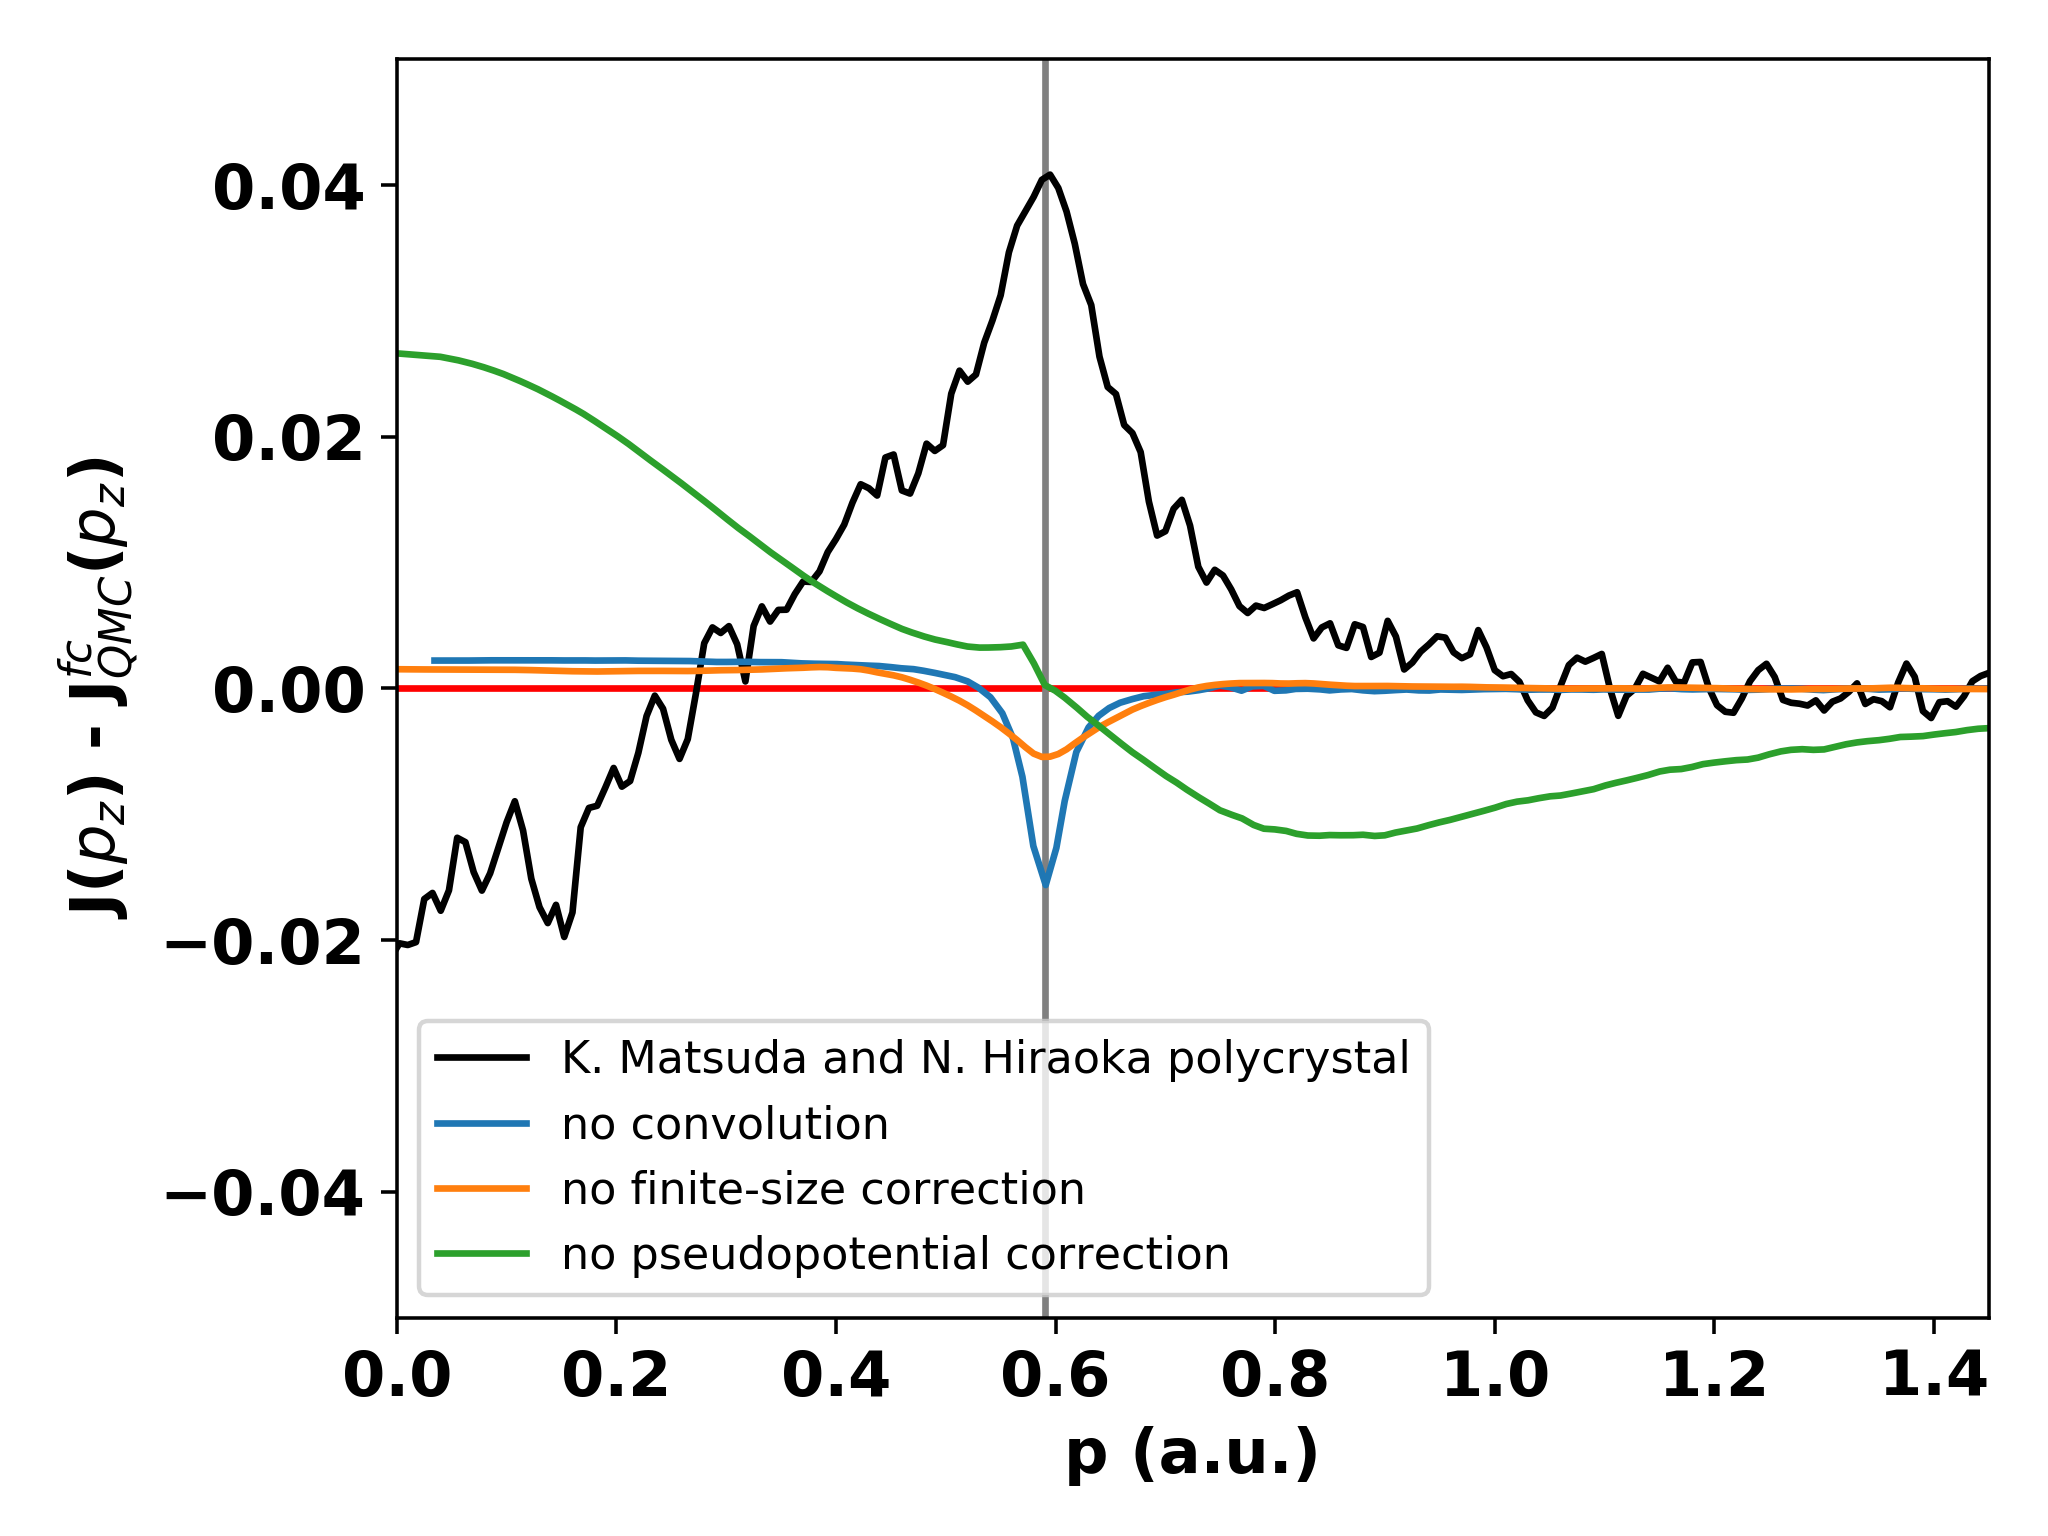
\includegraphics[scale=0.48]{figures/li40_fc7-djp-qmc}
\caption{Compton profile difference relative to best QMC result (red line in Fig.~\ref*{fig:crystal-vcp}). The black curve is experiment. The colored curves are $J(p)$ calculated with various approximations. The pseudopotential causes the largest bias (green curve).\label{fig:crystal-ppc}}
\end{figure}

\begin{comment}
\begin{figure}
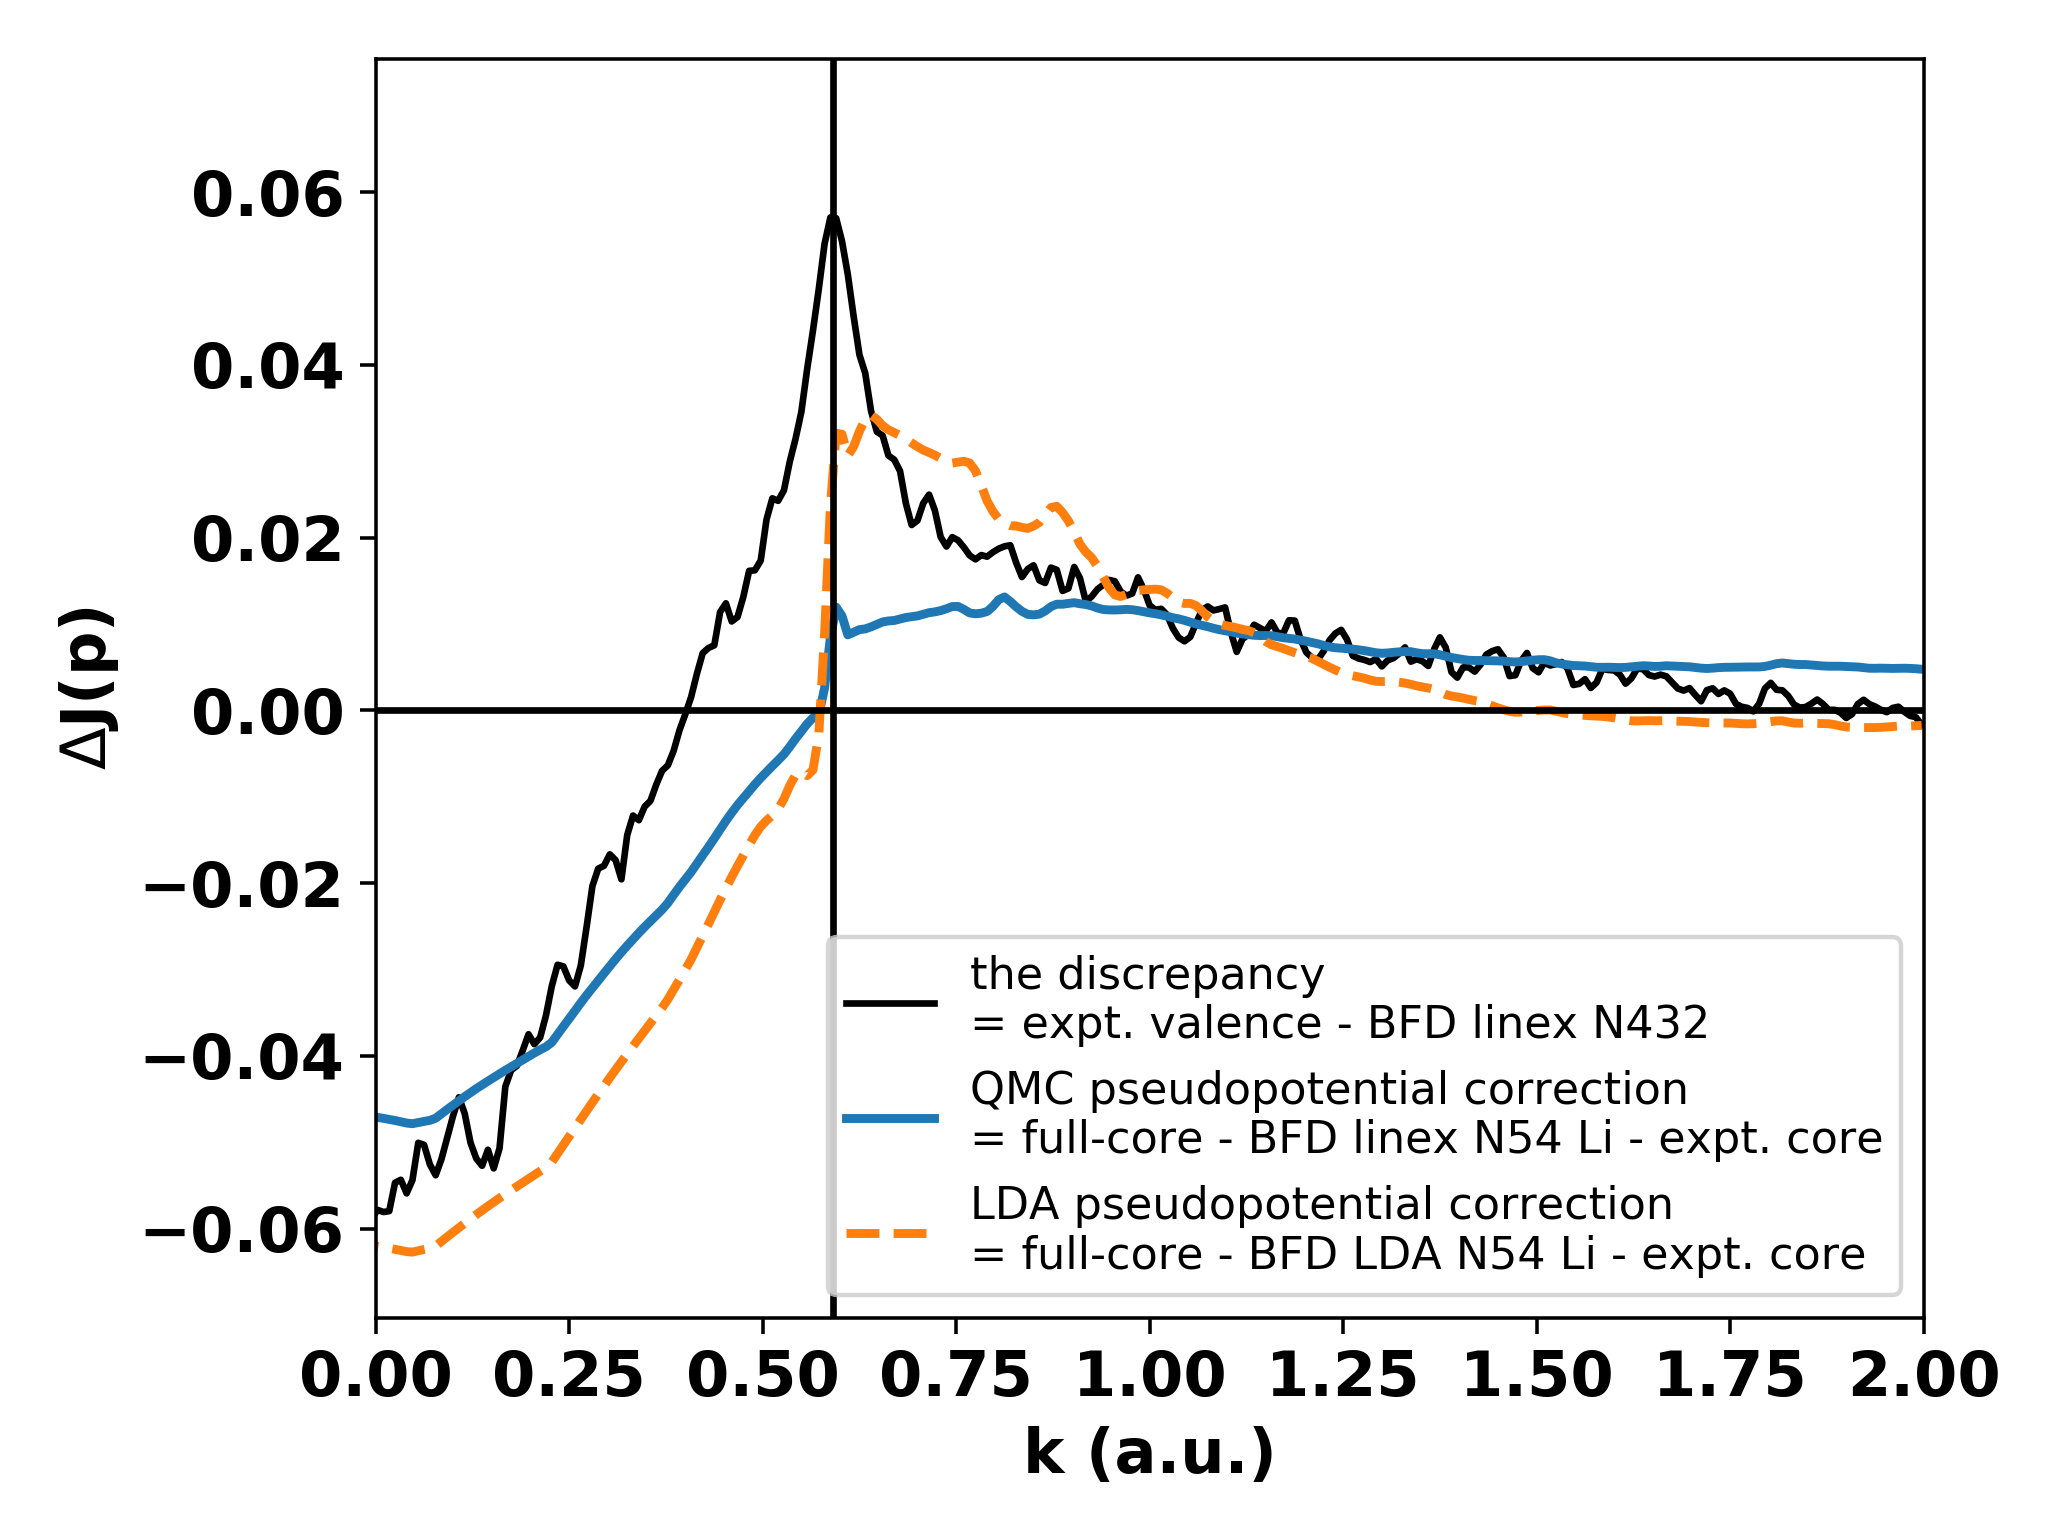
\includegraphics[scale=0.6]{figures/li40_fc5-jpv-ppc-linex}
\caption{The discrepancy between experiment and pseudopotential QMC Compton profile compared to pseudopotential correction derived from QMC (solid line) and DFT (dashed line). The black curve is the difference between the most recent experiment and our best pseudopotential calculation from Fig.~\ref{fig:crystal-vcp}. The black vertical line marks the Fermi momentum. The black horizontal line marks the experiment by K. Matsuda and N. Hiraoka. \label{fig:crystal-ppc}}
\end{figure}

A Compton profile pseudopotential correction is derived from the difference between all-electron and pseudopotential QMC \textcolor{red}{Compton profiles} for the 54-atom cell. This correction is shown alongside the discrepancy between the experiment and pseudopotential QMC Compton profile in Fig.~\ref{fig:crystal-ppc}. An equivalent pseudopotential correction can be derived from the LDA Compton profiles and is shown as the dashed line in Fig.~\ref{fig:crystal-ppc}. The pseudopotential correction accounts for the majority of the discrepancy between experiment and pseudopotential QMC away from the Fermi surface.
\end{comment}

In Fig.~\ref{fig:sl-jp-djp}, we show the QMC Compton profiles in the disordered solid and the liquid phases. %Both pseudopotential and corrected Compton profiles are shown. The QMC profiles are smoothed by convolution. In both cases, the pseudopotential-corrected profiles agree better with experiment. Further, the pseudopotential liquid Compton profile agrees better with experiment than its solid counterpart.

The main difference between the liquid and the solid momentum distributions is the absence of secondary Fermi surfaces caused by Umklapp processes. %The fact that liquid Compton profile agrees better with experiment corroborates the idea that the pseudopotential bias is significant. Namely, Umklapp processes involve the core electrons, which are replaced by a pseudopotential. The weaker the Umklapp, the less important the pseudopotential, and the smaller the bias.

\begin{figure*}[ht]
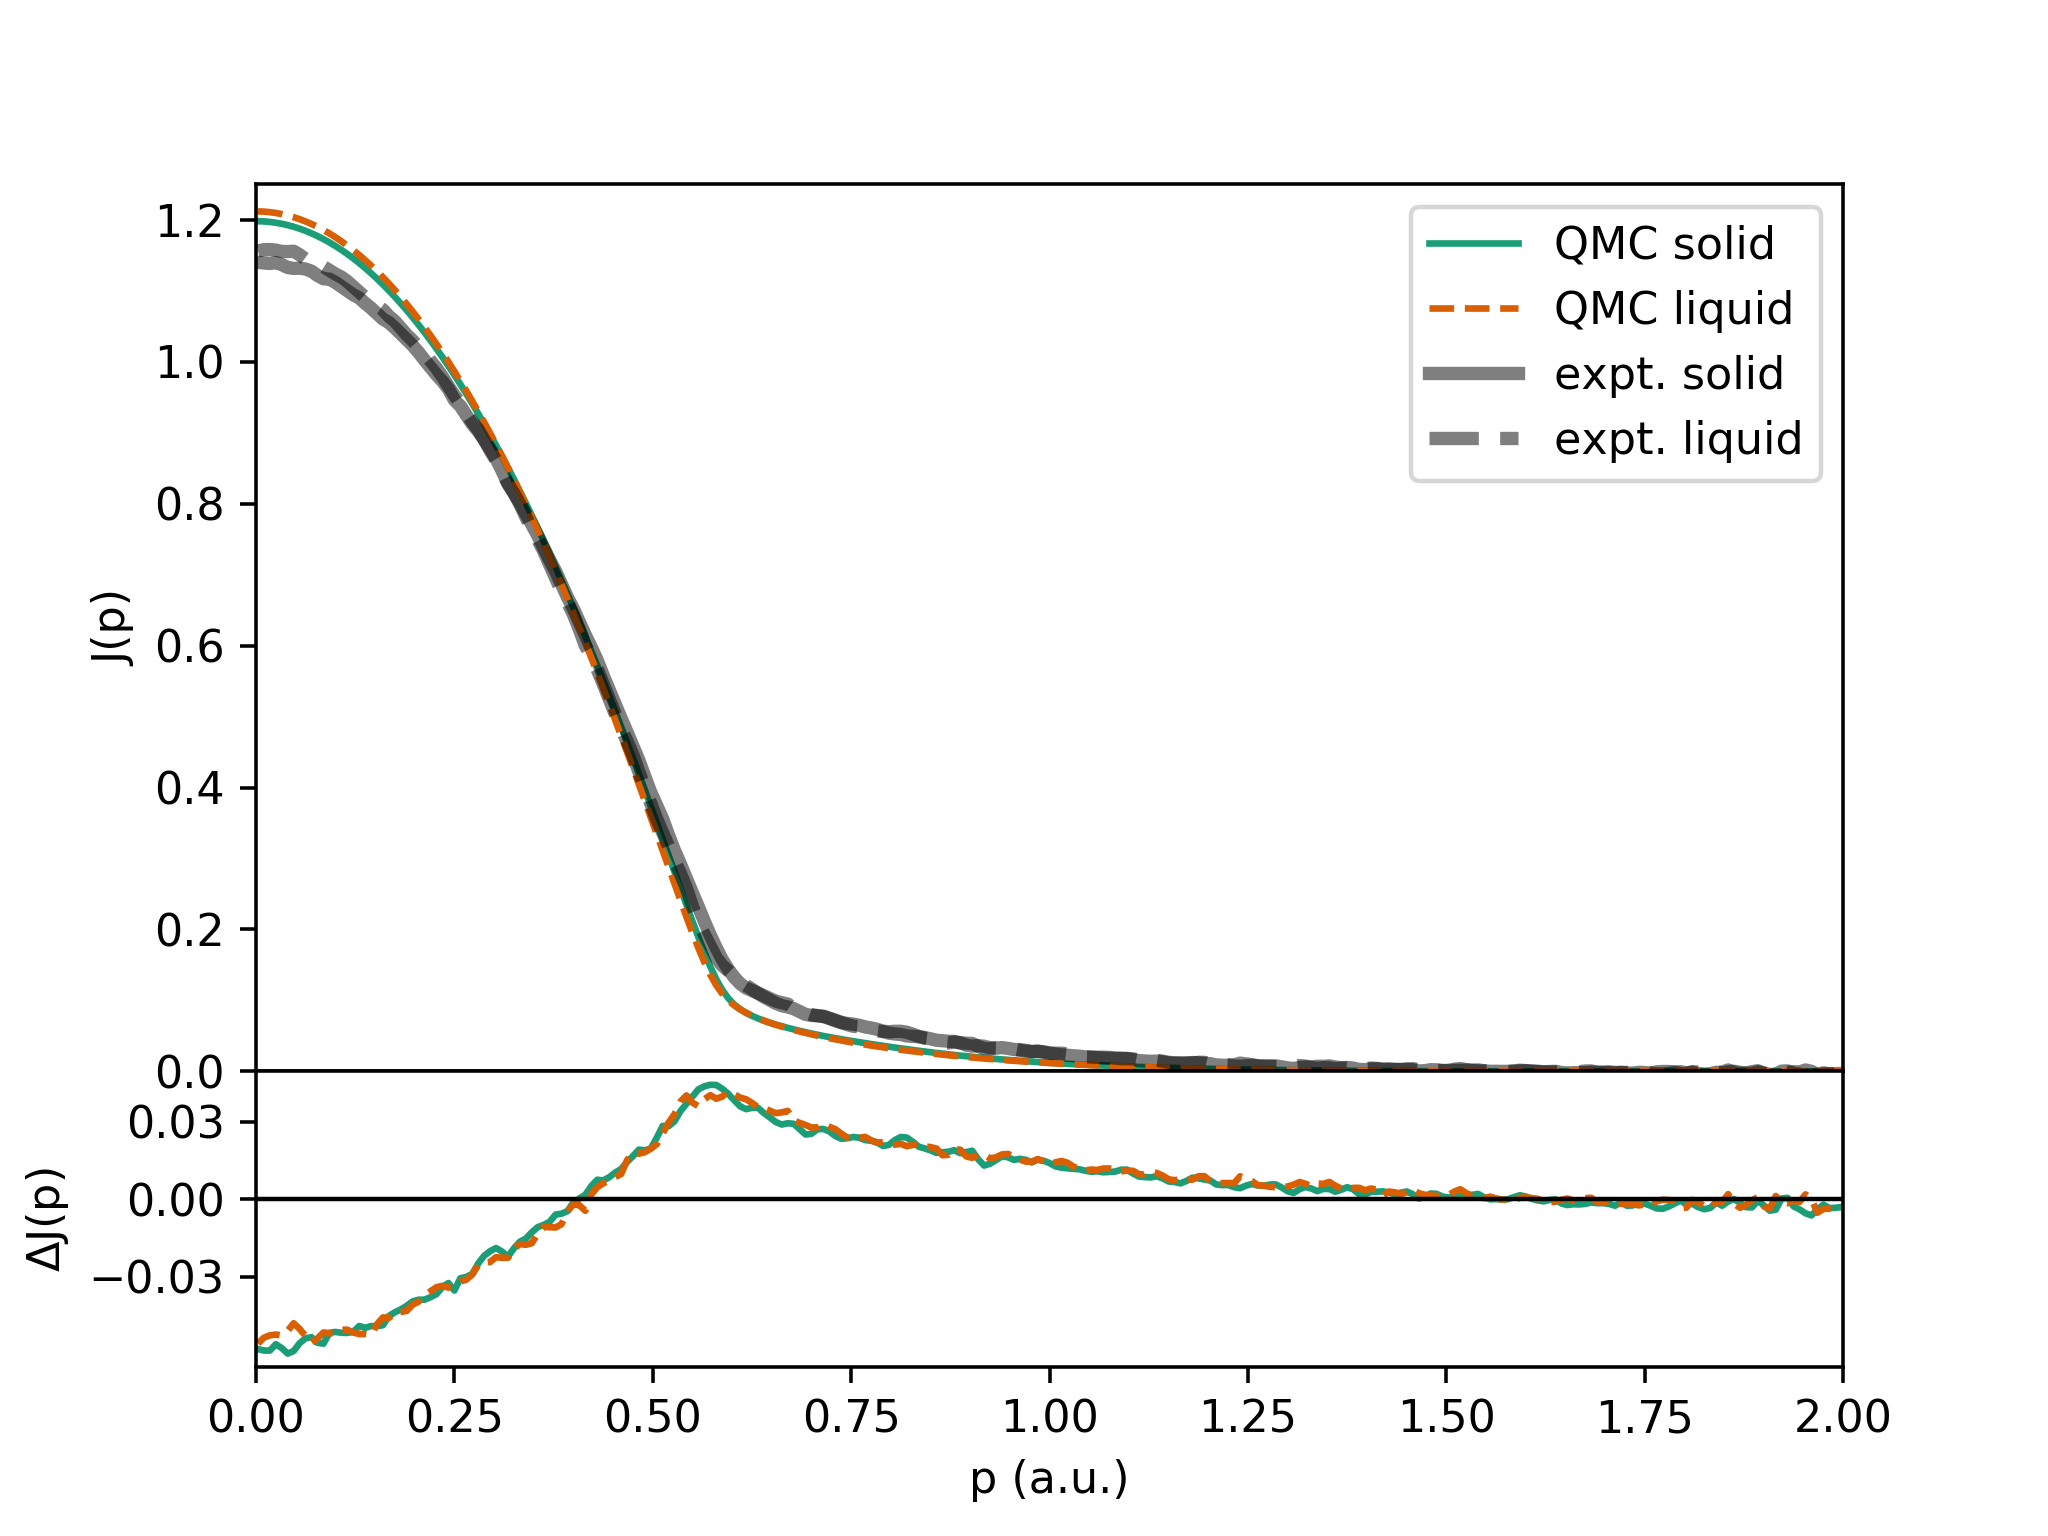
\includegraphics[scale=0.49]{figures/li52e_sl-jp}
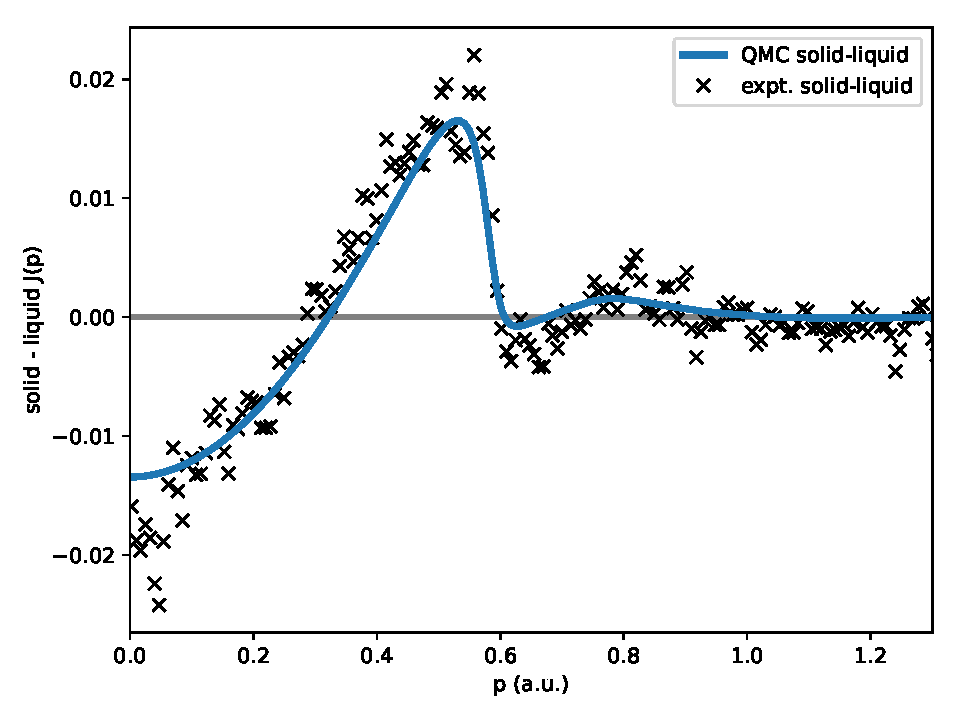
\includegraphics[scale=0.49]{figures/li52e_sl-djp}
\caption{solid and liquid lithium Compton profiles from QMC and experiment.\label{fig:sl-jp-djp}}
\end{figure*}

As shown in Fig.~\ref{fig:sl-jp-djp}, the remaining discrepancy between the pseudopotential-corrected QMC and experiment Compton profiles is on the order of 0.01 a.u. and peaks around the Fermi momentum.

\section{Discussion} \label{sec:discussion}

In the following, we discuss possible explanations for the remaining discrepancy in Fig.~\ref{fig:sl-jp-djp}. %The possibilities can be grouped into two conceptual categories: 1. imperfect inclusion of an effect we have considered; 2. the omission of an effect we have not considered. In the first category, we have considered correlation, thermal disorder, finite-size, and final-state interaction. In the second category, we have not considered the effect of thermal expansion, electronic thermal excitation, relativistic effects, and changes in the shape and location of the Fermi surface.

\emph{electron-ion correlation} - When treated as point charges, the crystal lattice mainly introduces inhomogeneity to an otherwise homogeneous valence electron density. Umklapp processes send electronic momentum density to secondary Fermi surfaces, thereby enhancing the high-momentum components of the momentum distribution. Due to the normalization sum rule, the momentum distribution is also lowered within the Fermi surface. Further, its discontinuity at the Fermi surface is reduced~\cite{P.EisenbergerL.LamP.M.Platzman1972}. In the absence of other interactions, the ground-state electronic density will be exact if the electron-ion correlation is perfectly captured.

DFT is designed to obtain the correct ground-state electronic density, so we expect it to include electron-ion correlation well. However, a pseudopotential is not designed to faithfully reproduce the charge inhomogeneity of the valence orbital in the core region. Therefore, pseudopotential introduces a bias in the valence momentum distribution. The qualitative effect of the pseudopotential is clear from its construction. When designing a pseudopotential, one smooths the valence orbital inside the core region. This will increase the electronic momentum density at low momenta (thus decrease it at high momenta to preserve normalization). Indeed, one can reproduce the overall trend of the pseudopotential correction by considering the smoothing of the pseudized valence orbital alone (Fig.~\ref{fig:hf-ppc}). We also see that augmented planewave (APW) calculations~\cite{Baruah1999,Bross2004,Bross2005,Bross2012} tend to reproduce the experimental Compton profiles better at low momenta than pseudopotential calculations.

\begin{figure}
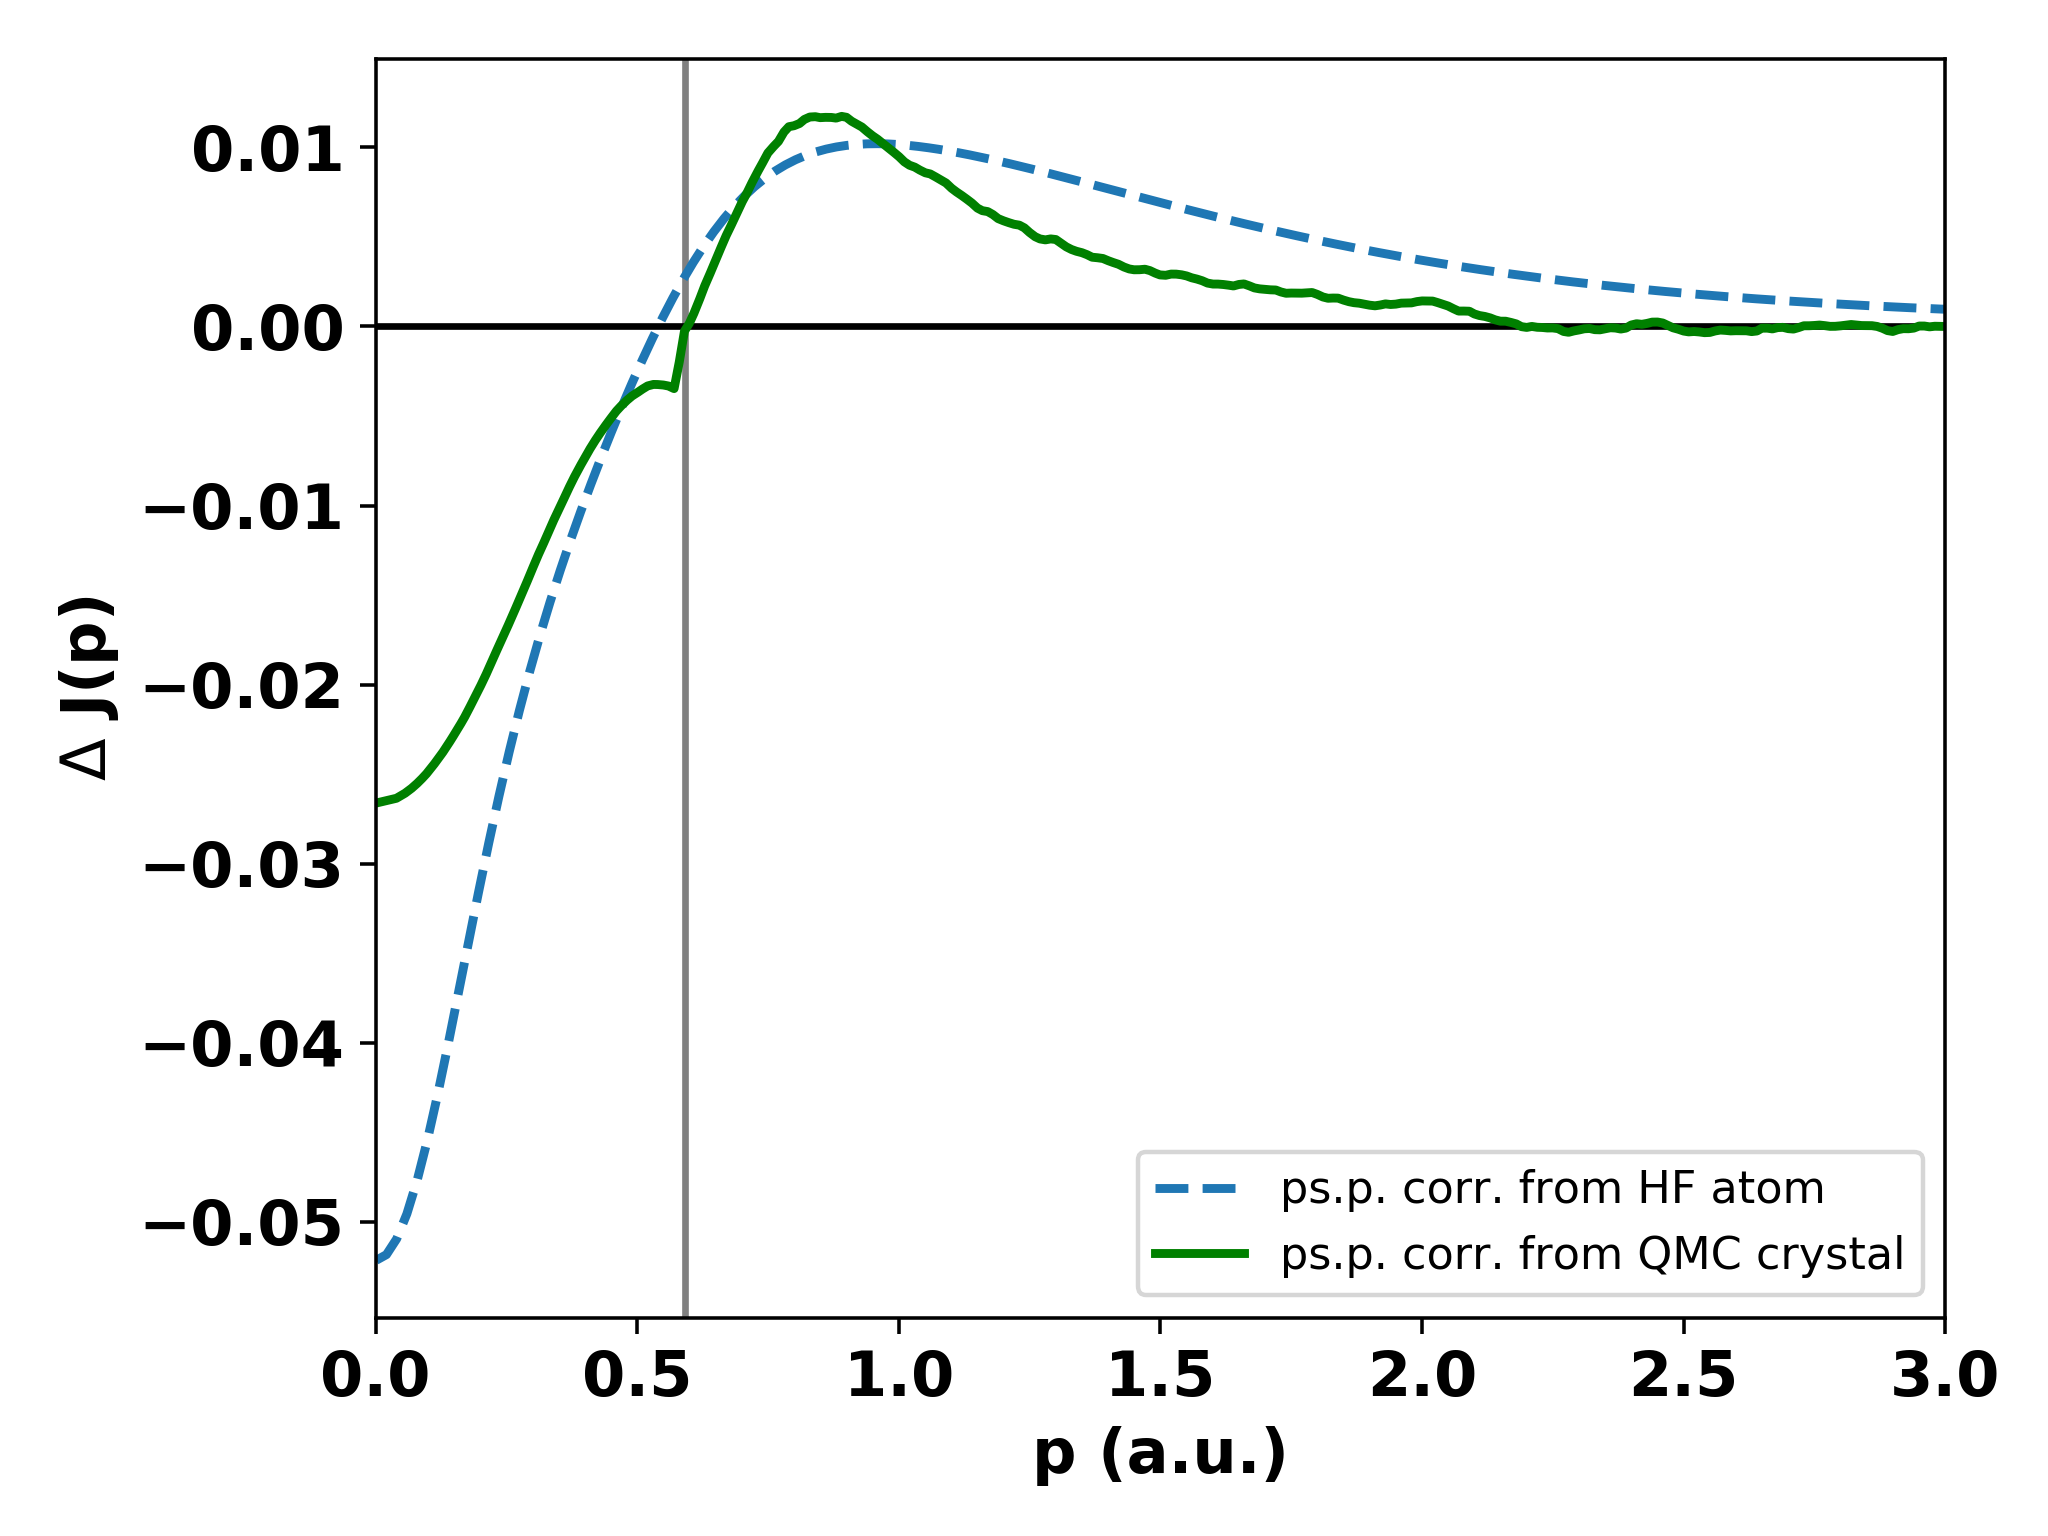
\includegraphics[scale=0.48]{figures/li42c_bfd-ppc}
\caption{Pseudopotential correction derived from QMC and HF. The green curve is the same QMC pseudopotential correction as shown in Fig.~\ref{fig:crystal-ppc}. The dashed blue curve is the pseudopotential correction derived from the all-electron v.s. pseudized lithium atom using HF. The gray vertical line marks the Fermi momentum. The black horizontal line marks zero.\label{fig:hf-ppc}}
\end{figure}

%QMC charge density is expected to be even more accurate than that from DFT. Firstly, VMC closely approximates the DFT charge density via the KS determinant. Secondly, DMC can fix up short-range correlation in a small amount of imaginary time. Therefore, we expect the QMC charge density to be accurate and well converged.

The pseudopotential correction is not perfect. It was derived in the perfect crystal, then applied to the disordered configurations. Ideally, one would directly perform all-electron QMC on the disordered configurations. However, this is computationally expensive. We do not consider all-electron calculation to be necessary in the solid phase, because the effect of disorder is small. The current pseudopotential correction does over-correct the liquid Compton profile at high momenta, because the corrections meant for the secondary Fermi surfaces are extraneous.

The corrected Compton profile in Fig.~\ref{fig:liquid-vjp} is in better agreement with experiment than its pseudopotential equivalent. Finally, the pseudopotential correction is concentrated around $p=0$. If it were underestimated, then the remaining correction would lower $J(0)$ much more than it would raise $J(p_F)$, worsening the agreement with experiment. Therefore, we think electron-ion correlation has been satisfactorily accounted for, and is not responsible for the remaining discrepancy.

\emph{disorder} - Disorder mostly reduces the effect of the crystal lattice, because deviations from the perfect lattice weakens Umklapp processes. A confirmation was obtained when Sternemann et. al. reproduced the temperature effect on the Compton profile of lithium by smearing out the pseudopotential with a Debye-Waller factor~\cite{Sternemann2001}.

Thermal disorder is also unlikely to be responsible for the remaining discrepancy because disorder-correction is small at the scale of the remaining correction. This can be seem by comparing the discrepancy in the perfect crystal (Fig.~\ref{fig:crystal-ppc}) to the discrepancy in the disordered solid (Fig.~\ref{fig:djp-remaining}). The two remaining discrepancies are similar in both shape and magnitude.

%Thermal disorder and thermal expansion can also contribute to the remaining discrepancy. The main effect of thermal disorder is to smear out the reciprocal lattice and suppress Umklapp processes~\cite{Sternemann2001}. This transfers electron momentum density from the secondary Fermi surfaces back to the main one, thus narrowing the Compton profile.

\emph{electron-electron correlation} - The effect of electron-electron (ee) correlation on the momentum distribution is similar to electron-ion correlation in that it increases high-momentum components, decreases low-momentum components and reduces the discontinuity at the Fermi surface. However, electron-electron correlation does not introduce secondary Fermi surfaces. While the effect of correlation is encoded in the LDA functional in DFT, ee correlation is completely absent from the KS determinant wavefunction. The Slater-Jastrow wavefunction can be thought of as a first-order modification of the free-electron Slater determinant by the Coulomb interaction~\cite{Holzmann2003}. Therefore, the Slater-Jastrow wavefunction captures correlation in a rigorous and rather natural manner. The Slater-Jastrow wavefunction does not capture all correlation effects and puts a bias on the DMC momentum distribution due to fixed-node error and mixed-estimator bias. However, we expect the Slater-Jastrow wavefunction to be accurate for simple metals. Further, it can be systematically improved, for example by a back flow transformation.
%Going to second order, we have back flow correlation as well as three-body Jastrow.

Remaining correlation effect is unlikely to be the main cause of the remaining discrepancy because the isotropic Lam-Platzman correction derived from the homogeneous electron gas was shown to be accurate by QMC~\cite{Filippi1999,Bross2005}. Further, the correlation correction of the LDA Compton profile is a relatively smooth function of momentum with a peak of magnitude $\sim$0.05 a.u. at the Fermi momentum. It seems unlikely that the remaining correlation correction to the QMC Compton profile would be of the same magnitude.

%Bross found that the Lam-Platzman correction is sensitive to the underlying model of the homogeneous electron gas~\cite{Bross2005}.

\emph{finite size} - Finite-size effects are more challenging to deal with in a many-body simulation than in a band structure calculation. In the DFT calculation of a perfect crystal, finite system size has no influence on the value of the momentum distribution at any momentum. Calculation performed in a larger simulation cell simply makes the momentum-space grid denser. In contrast, finite system size increases the magnitude of the discontinuity at the Fermi surface in QMC. Further, finite-size effect was found to diminish slowly with system size in the homogeneous electron gas~\cite{Holzmann2009}. Remaining finite-size correction is a likely explanation for at least a part of the remaining discrepancy, because finite-size correction peaks around the Fermi momentum, consistent with the discrepancy.

\emph{Fermi surface} - The Fermi surface of BCC lithium is anisotropic with pronounced secondary features. The KS-LDA main Fermi surface is a mesh of octagons facing [100], [110], triangles facing [111], and square patches to close the surface. The whole surface curves to approximate a sphere, somewhat like a soccer ball. Further, there is a clear secondary Fermi surface along the [110] direction at $p=(0.6, 0.6, 0)$ a.u.. The position and shape of the KS-LDA Fermi surface are preserved in the QMC simulation. If the Fermi surface geometry is slightly different in reality, then the ensuring bias on the momentum distribution will peak at the Fermi momentum. Therefore, the position and shape of the LDA Fermi surface is another possible explanation of the remaining discrepancy.

\emph{\textcolor{red}{density change}} - Electron density change is an important effect to consider because it changes the valence electronic density and moves the Fermi surface. Electron density can change due to thermal expansion and phase transition (from solid to liquid for example). E. Klevak et. al. showed that upon raising temperature from 0 to 300K, the Compton profile narrows and $J(0)$ increases by $\sim$ 0.025 a.u.~\cite{Klevak2016}. The experimental Fermi momenta for the solid and liquid states are 0.595 and 0.585 a.u., respectively. They correspond to homogeneous valence densities of $r_s=3.225$ and $r_s=3.28$, which differ slightly from the density $r_s=3.25$ used in our calculations.

Thermal expansion is a likely explanation for much of the remaining discrepancy in the solid state. The effect of expanding a spherical Fermi surface from $p_F=0.590$ ($r_s=3.25$) to $p_F=0.595$ a.u. ($r_s=3.225$) on the Compton profile is similar to the remaining discrepancy (Fig.~\ref{fig:djp-remaining}) in both shape and magnitude. On the other hand, thermal expansion will worsen the agreement between QMC and experiment in the liquid state.

\emph{final state} - Last but not least, the ``impulse approximation'' is known to be inaccurate for core electrons and cause asymmetric in the measured Compton profile~\cite{Eisenberger1970,Sternemann2000,Huotari2001}. To go beyond the ``impulse approximation'', one must consider interaction of the scattered electron with the rest of the system in the final state. Final-state effects arise from two physical interactions. The first is the interaction between the excited quasi-particle with its surrounding medium. The second is the interaction between the excited quasi-particle and the hole it lefts behind. C. Sternemann et. al. showed that the self-energy combined with the vertex correction can satisfactorily explain the asymmetry of the Compton profile~\cite{Sternemann2000}. The effect of final-state interaction on the Compton profile can be approximated by convolving the spectral density function of the excited electron with the ground-state Compton profile. This convolution smears out the derivative-discontinuity of the Compton profile at the Fermi momentum. Thus the convolution correction also peaks at the Fermi momentum.

We accounted for final-state effects by convolving the QMC Compton profiles with a model function provided to us by N. Hiraoka [private communication]. The model function is an accurate representation of the convolution of the experimental resolution function and the spectral density function of the excited particle in the final state~\cite{Soininen2001}.

Final-state effect is unlikely to be the main cause of the remaining discrepancy, because the convolution correction is small on the scale of the discrepancy shown in Fig.~\ref{fig:crystal-ppc}. Further, the convolution correction is insensitive to small adjustment of parameters in the model function.

%We found that if the pseudopotential QMC Compton profiles were convolved with a Lorentzian having FWHM $\Gamma=0.026$ a.u., then they would agree almost perfectly with experiments. We believe this agreement is rather fortuitous. The long tail of the Lorentzian happens to be able to model the effect of the pseudopotential at $p=0$ and the remaining smearing at $p=p_F$ simultaneously.

% hypothesis: the slow varying background is due to the failure of the IA. The peak at Fermi momentum is due to remaining correlation and finite-size errors.

\section{Conclusion and Outlook}

%Significant advances in both theory and experimental techniques have brought the QMC and synchrotron X-ray Compton profiles of lithium to near perfect agreement.
Leveraging new algorithm and hardware, we improved the QMC Compton profile of lithium and provided the first QMC results in the disordered solid and the liquid states. Our QMC Compton profiles of the disordered solid and the liquid agree very well with the most recent synchrotron experiment. We resolved the discrepancy between pseudopotential QMC and experiment at zero and high momenta using an all-electron QMC calculation. We discussed potential explanations for the remaining discrepancy, which is concentrated at the Fermi surface. Future studies should give substantial consideration to effects beyond electron-electron correlation. Fermi surface shape and final-state effect are of particular interest.%, because the ensuing change to the Compton profile will be concentrated at the Fermi surface.

Current state-of-the-art QMC algorithms are ready to aid synchrotron experiments in understanding the measured Compton profiles. It would be interesting to revisit the challenging problem that is the 3D reconstructing of the momentum distribution from directional Compton profiles~\cite{Schulke1996,Tanaka2001}. Momentum resolution has been increased by new techniques in both theory and experimental. Further, all-electron QMC is feasible for perfect crystals in supercells containing thousands of electrons. The comparison between beryllium and lithium will be particularly interesting, because they have the same crystal structure but very different electron-ion interactions~\cite{P.EisenbergerL.LamP.M.Platzman1972}. A detailed study of these systems can shed more light on the nature of electron-ion and perhaps the electron-phonon interactions in simple metals.

Finally, when sufficient accuracy has been achieved in both theory and experiment, one can study the difference between ground-state and final-state Compton profiles to extract information on the dynamic structure factor of the system.

\section{Acknowledgment}

YY and DMC were funded by DOE 0002911. This work made use of the Blue Waters sustained-petascale computing project and the Illinois Campus Cluster, supported by the National Science Foundation (awards OCI-0725070 and ACI-1238993), the state of Illinois, the University of Illinois at Urbana-Champaign and its National Center for Supercomputing Applications. We would like to thank Kazuhiro Matsuda and Nozomu Hiraoka for sharing their experimental Compton profiles with us. We would like to thank Ilkka Kyl\"anp\"a\"a and Jaron Krogel for valuable discussions.

\begin{comment}
\section{Appendix}
The combined effect of finite experimental resolution and final-state interaction can be approximated by convolution with an extended Lorentzian
eq.~(\ref{eq:elorentz}) having FWHF $\Gamma=0.024$ a.u. and $a_1=0.85$, $a_2=0.05$
\begin{align}
\tilde{L}(x,\Gamma,a_1, a_2) = \frac{1}{\tilde{\Omega}} \frac{1}{
1+a_1(\frac{2x}{\Gamma})^2+a_2(\frac{2x}{\Gamma})^4
}.\label{eq:elorentz}
\end{align}
\end{comment}

\bibliographystyle{apsrev}
\bibliography{ref,qmc,basic}

\end{document}
